\documentclass{my-article}
\usepackage{my-coverpage}
\usepackage{my-codespace}

\usepackage[utf8]{inputenc}
\usepackage[T5]{fontenc}
\usepackage[vietnamese]{babel}

\usepackage{pdflscape}
\usepackage{pdfpages}

%\usepackage{textcomp}
% =========================
% Cover page information
% =========================

\NameUpperUniname{Vietnam National University Ho Chi Minh City}
\NameUniname{Ho Chi Minh City University of Technology}
\NameDeptname{Department of Electronics}
\NamePathlogo{./my-chapters/my-images/01_logobachkhoatoi.png}
\NameClass{Applied Electronics (EE3129)}
\NameGroup{02}
\NameLesson[\Large]{BIGPROJECT 2 REPORT}
\NameTitle[\Huge]{Thiết kế mạch đo nhiệt độ sử dụng Thermistor}
\NameAdvisor{Nguyễn Trung Hiếu}
\NamePlace{Ho Chi Minh}
\NameTime{../../20..}
\NamePathBackground[width=\paperwidth,height=\paperheight]{./my-chapters/my-images/bia.jpg} 
\MemberTableData{
1 & 2212904 & Đoàn Ngọc Sang & L02 & 100\% \\ \hline
2 & 2210780 & Nguyễn Đại Đồng & L02 & 100\% \\ \hline
3 & 2210164 & Trần Nguyễn Trâm Ánh & L02 & 100\% \\ \hline
}

% =========================
% Configuration
% =========================

\fancyhf{}
%\fancyhead[L]{\leftmark}
\newcommand{\finalresult}[1]{%
	\begin{tikzpicture}[baseline=(content.base)]
		\node[draw=red, thick, rounded corners=3pt, inner sep=6pt] (content)
		{\ensuremath{#1}};
	\end{tikzpicture}%
}
% =========================
% Document
% =========================
\begin{document}
\pagestyle{empty}
\MycoverFinalProject % Cover page
\newpage
\renewcommand{\arraystretch}{1.5}
\setlength{\parindent}{1cm}
\onehalfspacing
\setlength{\parskip}{6pt} 
\tableofcontents
\listoffigures
\listoftables
\listoflistings
\newpage
\pagestyle{fancy}
\MycountPages{number}
\fancyfoot[L]{
\includegraphics[width=.02\linewidth]{./my-chapters/my-images/logo_DEE.png}\text{Department of Electronics}}
\fancyhead[R]{GVHD: Nguyễn Trung Hiếu}

\newpage

\section*{Đề tài 4} 

Thiết kế mạch đo nhiệt độ sử dụng Thermistor. Mạch có tầm đo $20 - 80 ^{o}C$, độ phân giải $0.1^{o}C$, ngõ ra là điện áp tương ứng từ $0-5\,\textsf{V}$:
\begin{enumerate}[label=\arabic*.]
	\item Lựa chọn và mô phỏng Thermistor 2 dây (có điện trở dây dẫn là $10\,\Omega$).
	\item Lựa chọn điện trở song song để tuyến tính hóa.
	\item Lựa chọn OPAMP sử dụng, mô phỏng OPAMP theo datasheet.
	\item Đảm bảo sai số (giữa giá trị lý thuyết và thực tế đo qua mạch) $\pm 5\%$.
	\item Thiết kế mạch đọc điện áp cho ngõ ra ADC. Tiến hành lựa chọn ADC (số bit, nguồn). Mô phỏng mạch đọc và kiểm chứng.
\end{enumerate}

\section{Thực hiện mạch đo nhiệt độ}

\subsection{Mô phỏng trên Multisim}
\begin{figure}[H]
	\centering
	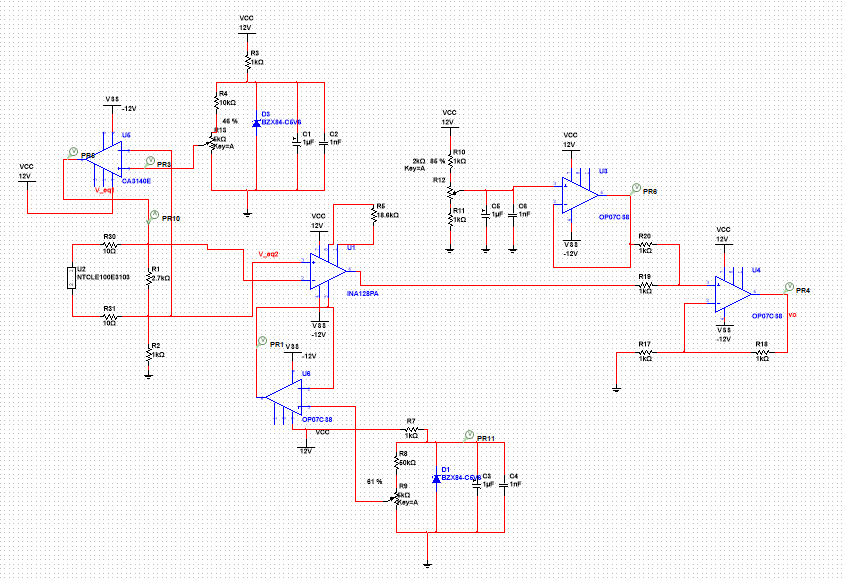
\includegraphics[width=0.7\linewidth]{my-chapters/my-images/Circuit_sim/overview_mul}
	\caption{Schematic Nmultisim}
	\label{fig:overviewmul}
\end{figure}

\begin{itemize}[label=-]
	\item Để tạo các điện áp tham chiếu 1V và 0.2V nhóm sử dụng diode zenner BZX84C5V6 có điện áp ngược ổn định 5.6V.
	\item Bỏ bớt 1 opamp giữa INA128 (U1) và ) OP7CS8 ( U4) có vai trò như 1 bộ đệm vì điều này ko cần thiết tốn tài nguyên.
\end{itemize}

\begin{figure}[H]
	\centering
	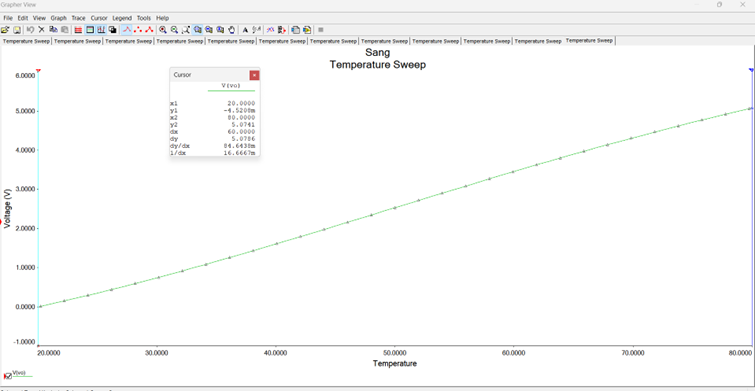
\includegraphics[width=0.7\linewidth]{my-chapters/my-images/Circuit_sim/sim_multisim}
	\caption{Mô phỏng trên Multisim}
	\label{fig:simmultisim}
\end{figure}

\subsection{Thực thi mạch trên Altium}

\subsubsection{Schematic}

\begin{figure}[H]
	\centering
	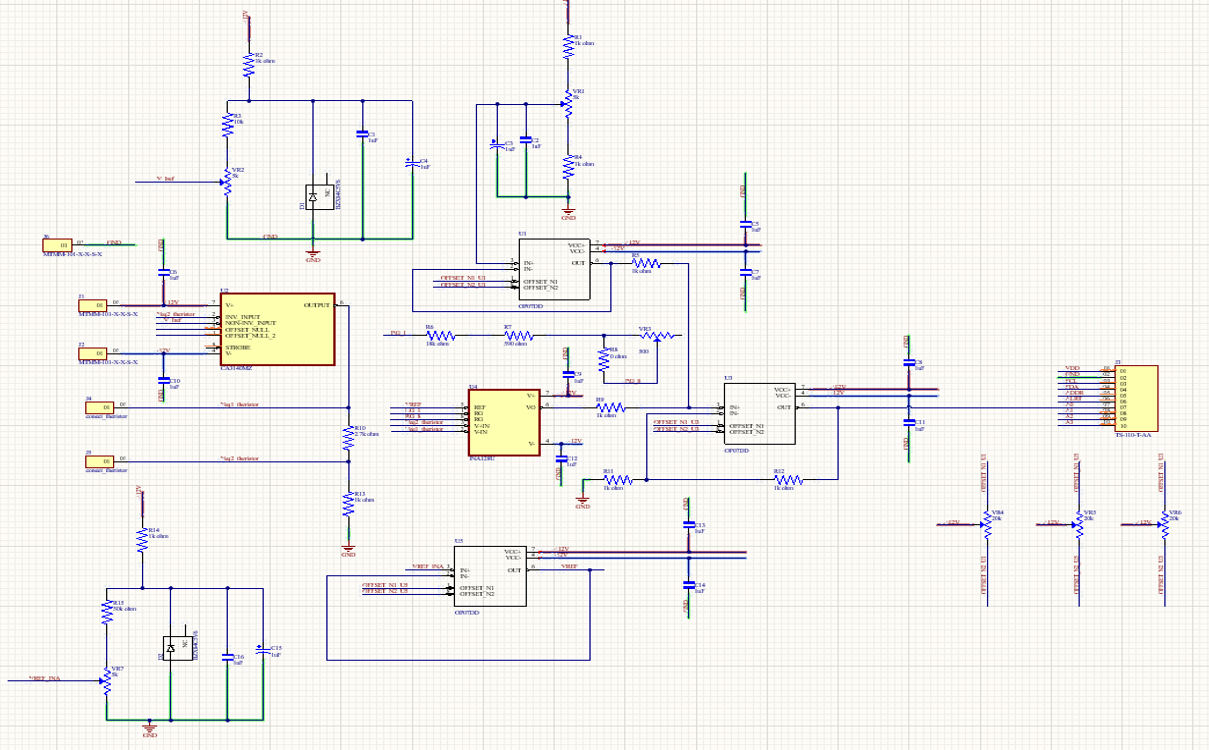
\includegraphics[width=0.8\linewidth]{my-chapters/my-images/Circuit_sim/PCB_schematic_sensor}
	\caption{Schematic của Mạch đọc nhiệt độ.}
	\label{fig:pcbschematicsensor}
\end{figure}

\subsubsection{Layout}

\begin{figure}[H]
	\centering
	\begin{minipage}{.45\linewidth}
		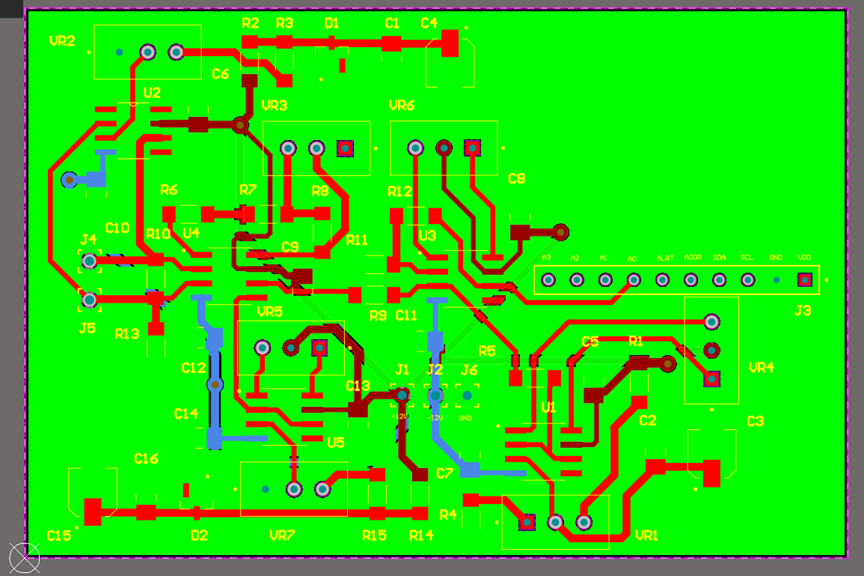
\includegraphics[width=\linewidth]{my-chapters/my-images/Circuit_sim/PCB_layout_sensor}
	\end{minipage}
	\begin{minipage}{.45\linewidth}
		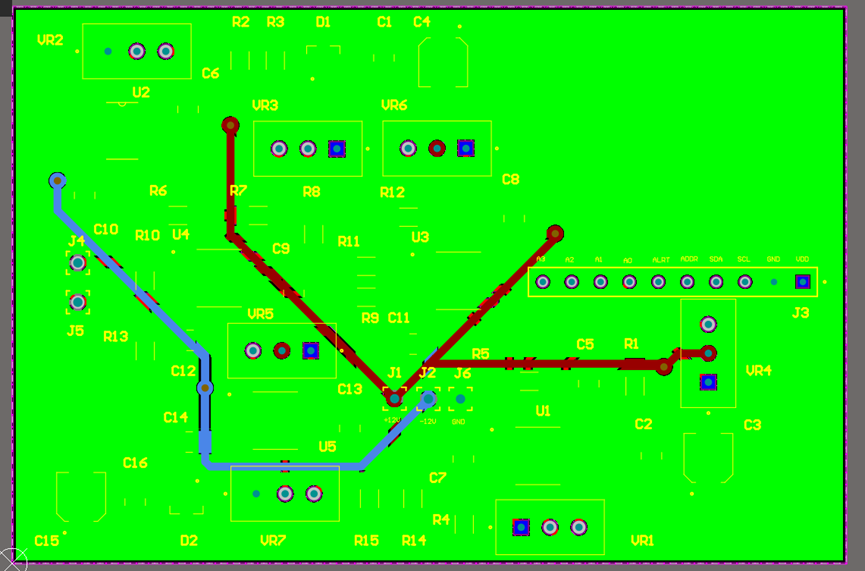
\includegraphics[width=\linewidth]{my-chapters/my-images/Circuit_sim/PCB_layout_sensor_1}
	\end{minipage}
	\caption{Layout của Mạch đọc nhiệt độ.}
	\label{fig:pcblayoutsensor}
\end{figure}

\begin{figure}[H]
	\centering
	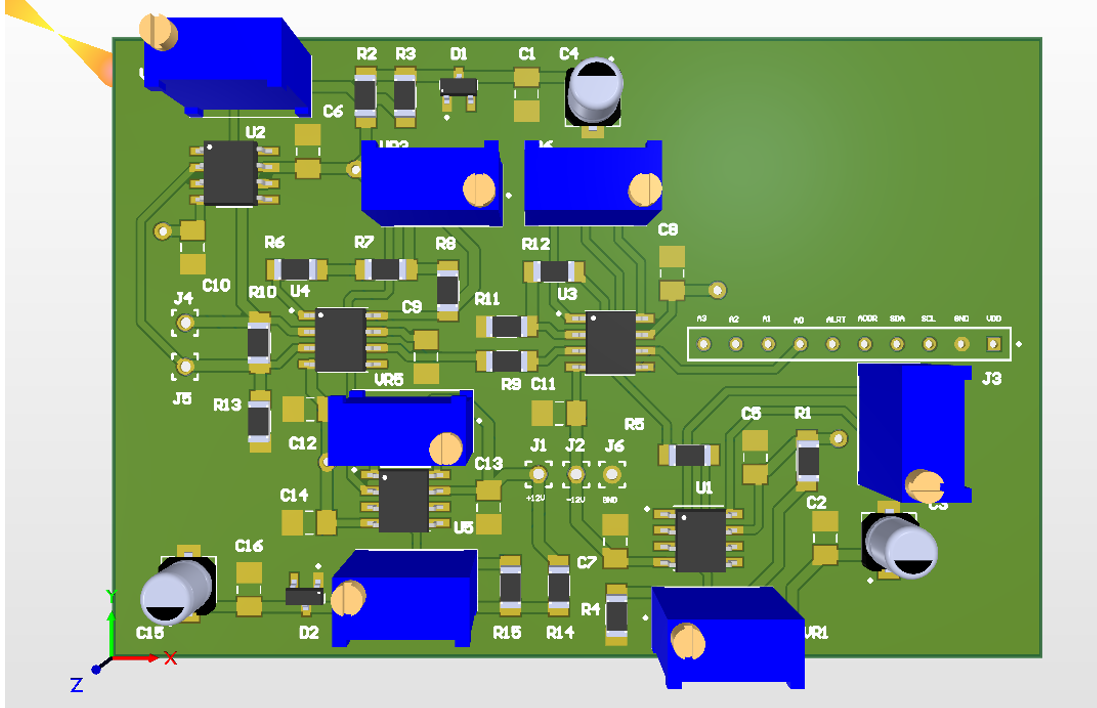
\includegraphics[width=0.7\linewidth]{my-chapters/my-images/Circuit_sim/PCB_3d}
	\caption{Mô hình 3D của Mạch đọc nhiệt độ.}
	\label{fig:pcb3d}
\end{figure}

\begin{figure}[H]
	\centering
	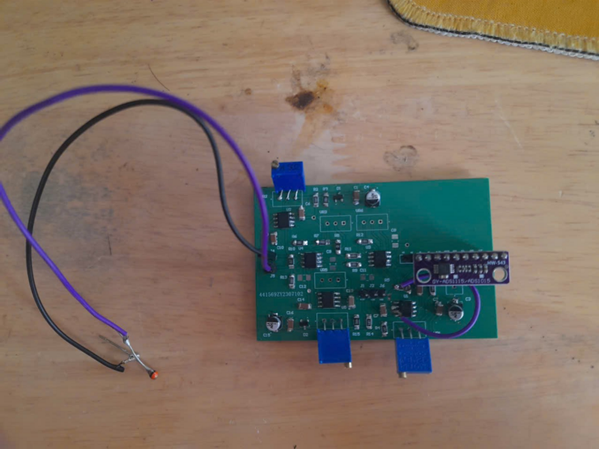
\includegraphics[width=0.7\linewidth]{my-chapters/my-images/Circuit_sim/PCB_thucte}
	\caption{Mạch thực tế của Mạch đọc nhiệt độ.}
	\label{fig:pcbthucte}
\end{figure}

\subsubsection{Thực hiện test mạch thực tế}

\begin{figure}[H]
	\centering
	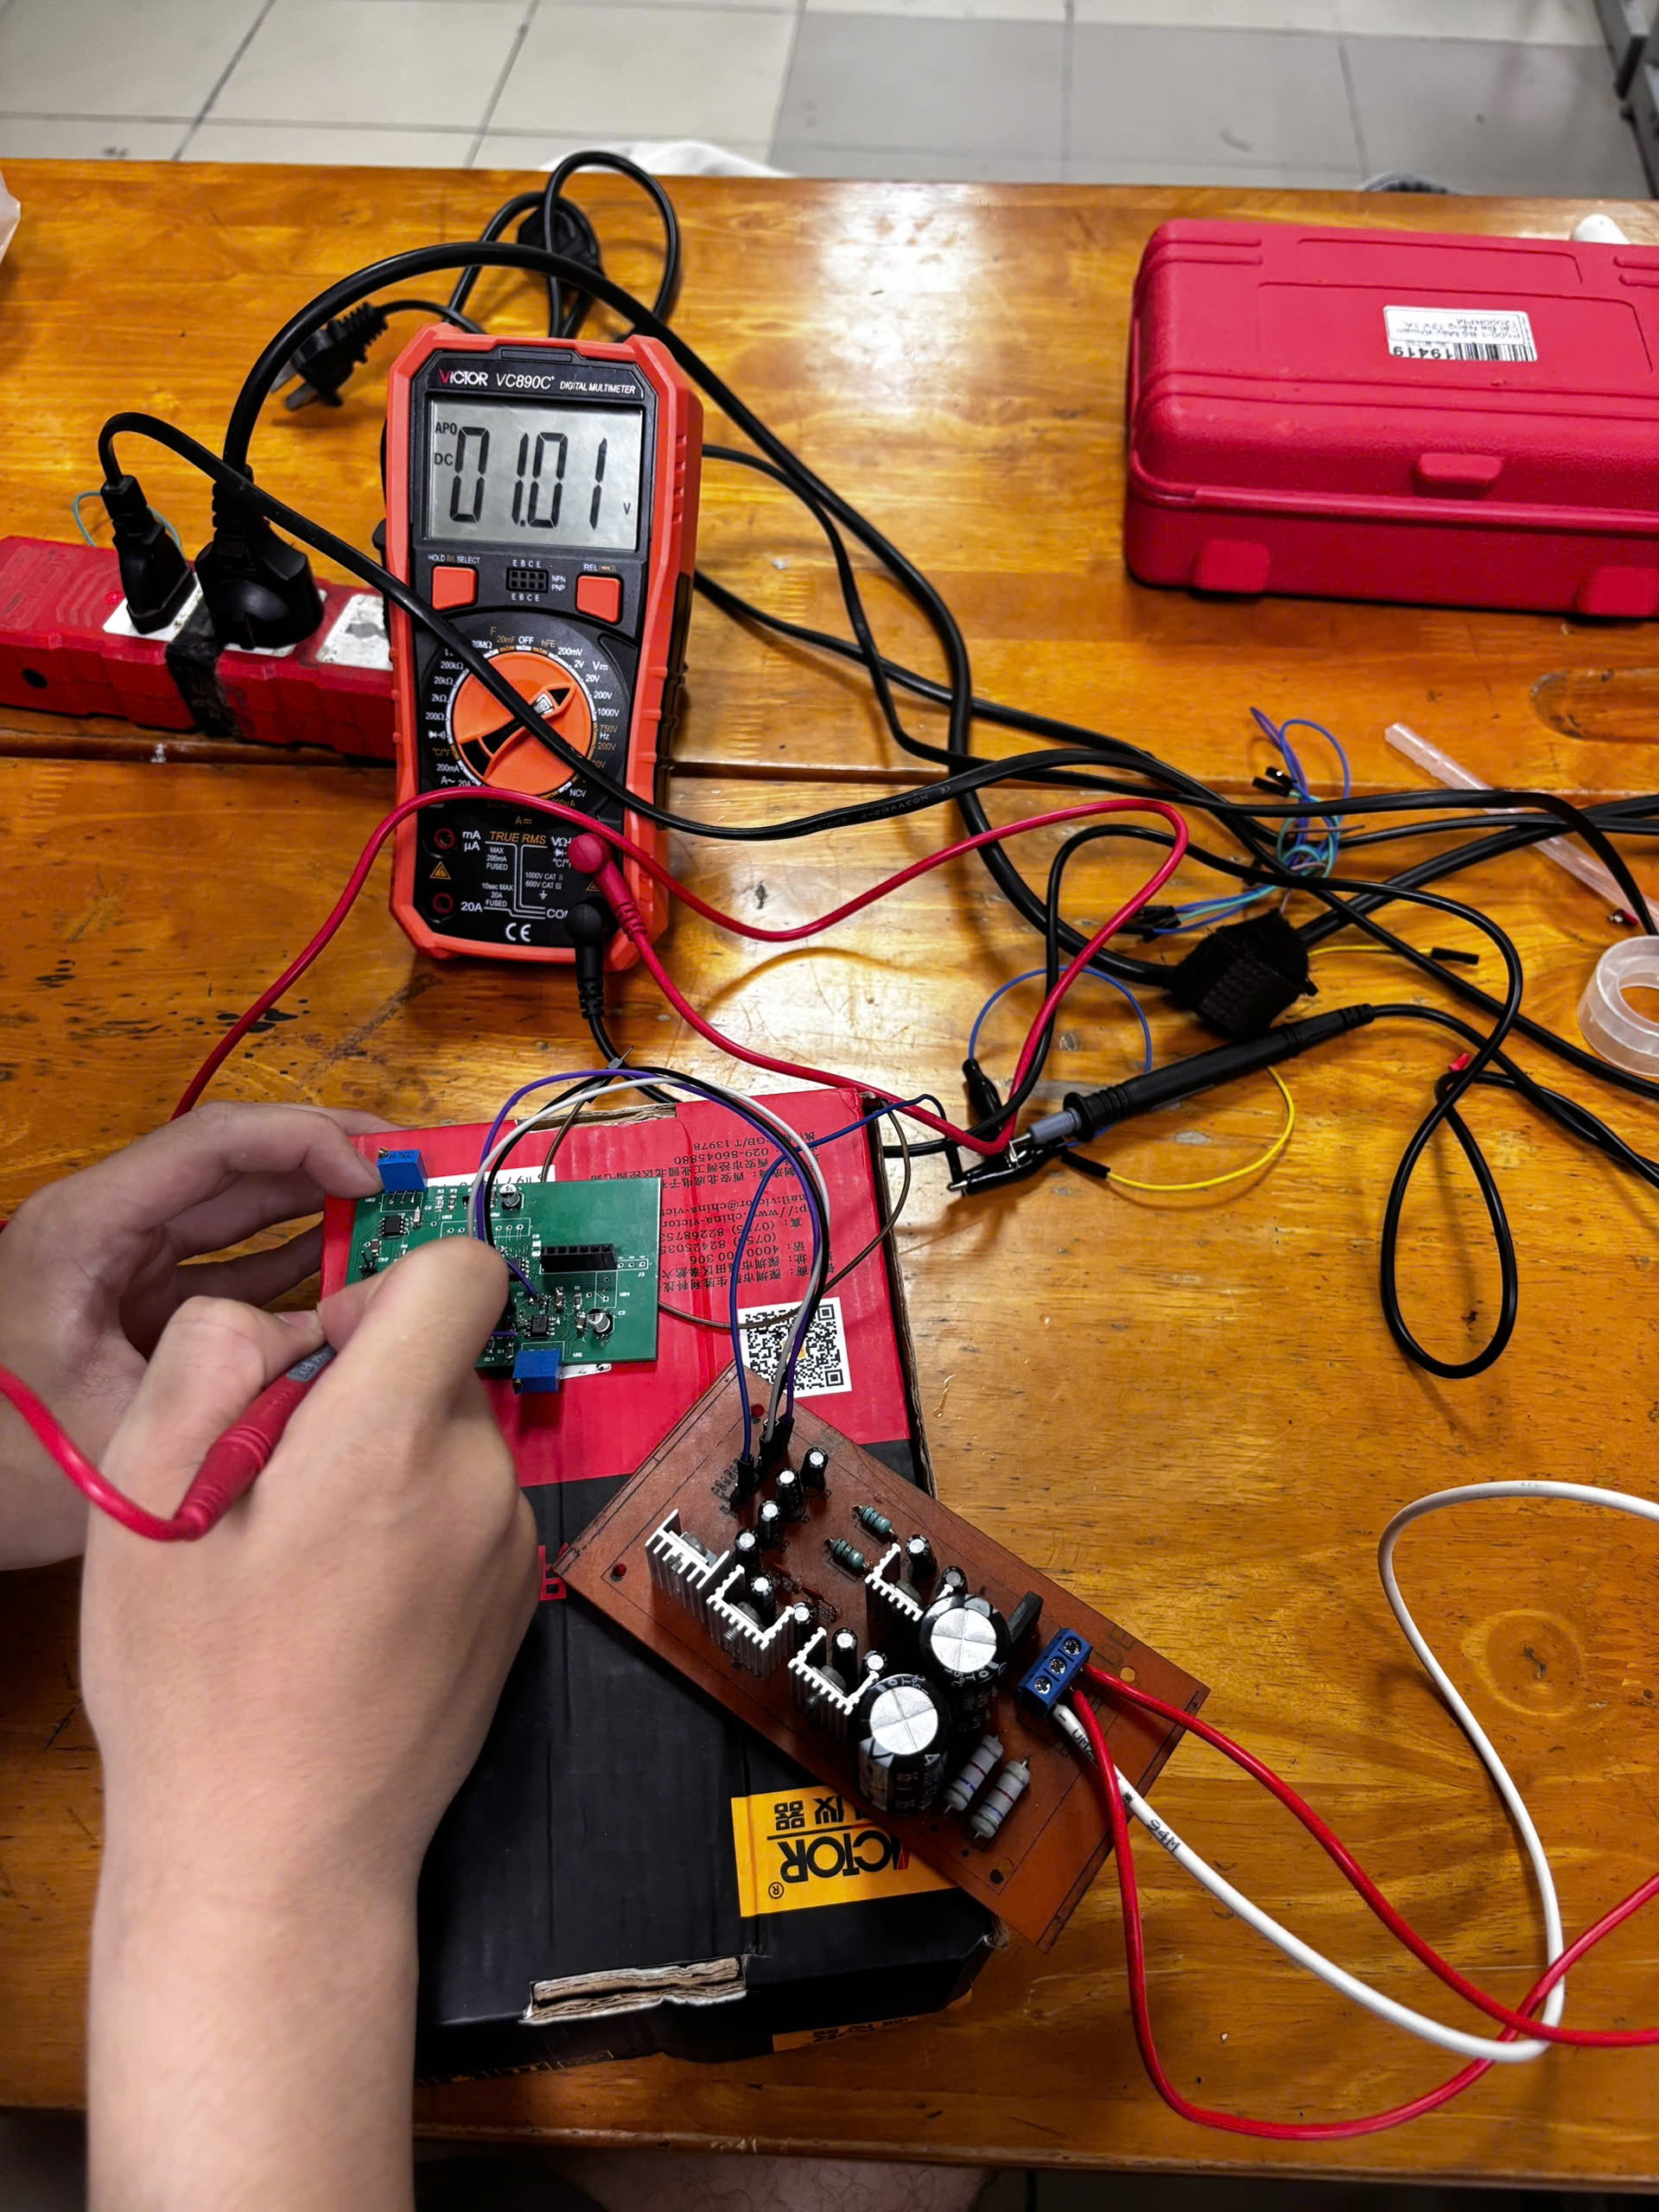
\includegraphics[width=0.7\linewidth]{my-chapters/my-images/Circuit_sim/CIRCUIT_1mA}
	\caption{Kiểm tra tạo nguồn dòng $1m\textsf{A}$.}
	\label{fig:circuit1ma}
\end{figure}

Ta thấy mạch đã tạo điện áp 1V ngay trên điện trở $1\textsf{K}\Omega$:

\begin{figure}[H]
	\centering
	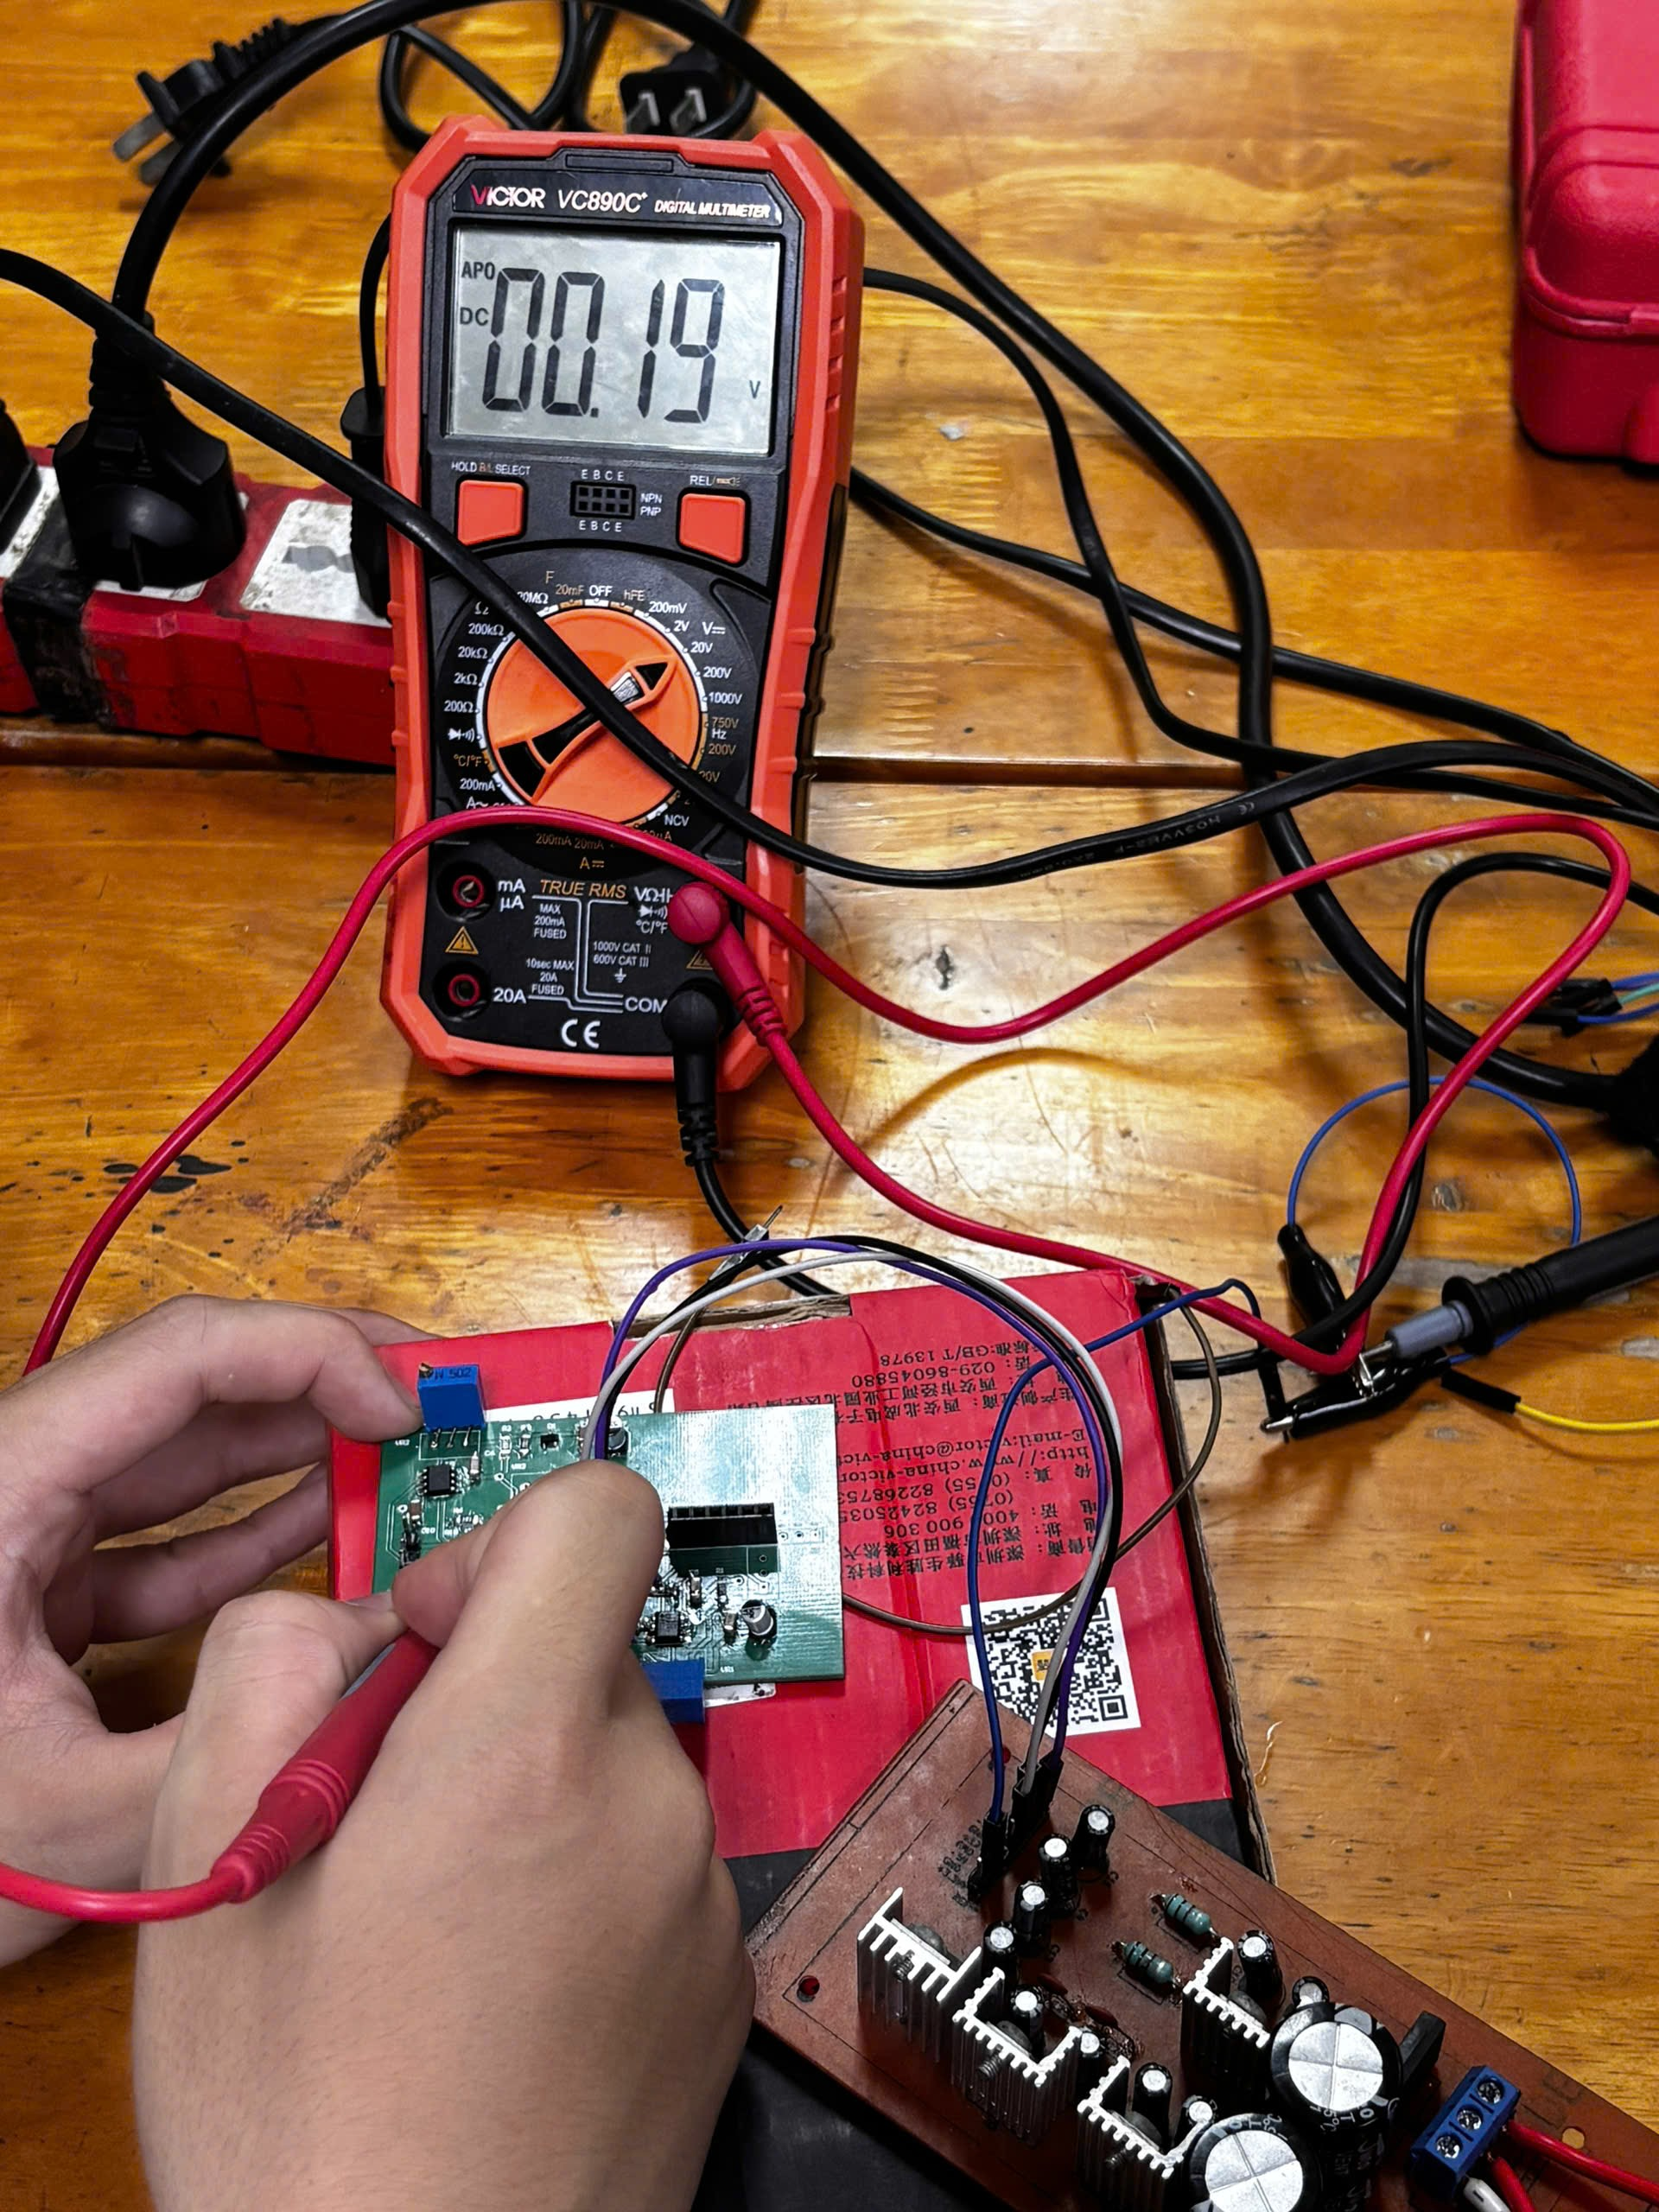
\includegraphics[width=0.7\linewidth]{my-chapters/my-images/Circuit_sim/CIRCUIT_0_2V}
	\caption{Kiểm tra mạch tao điện áp tham chiếu cho INA128 Theo lý thuyết là $0.2\textsf{V}$.}
	\label{fig:circuit02v}
\end{figure}

\begin{figure}[H]
	\centering
	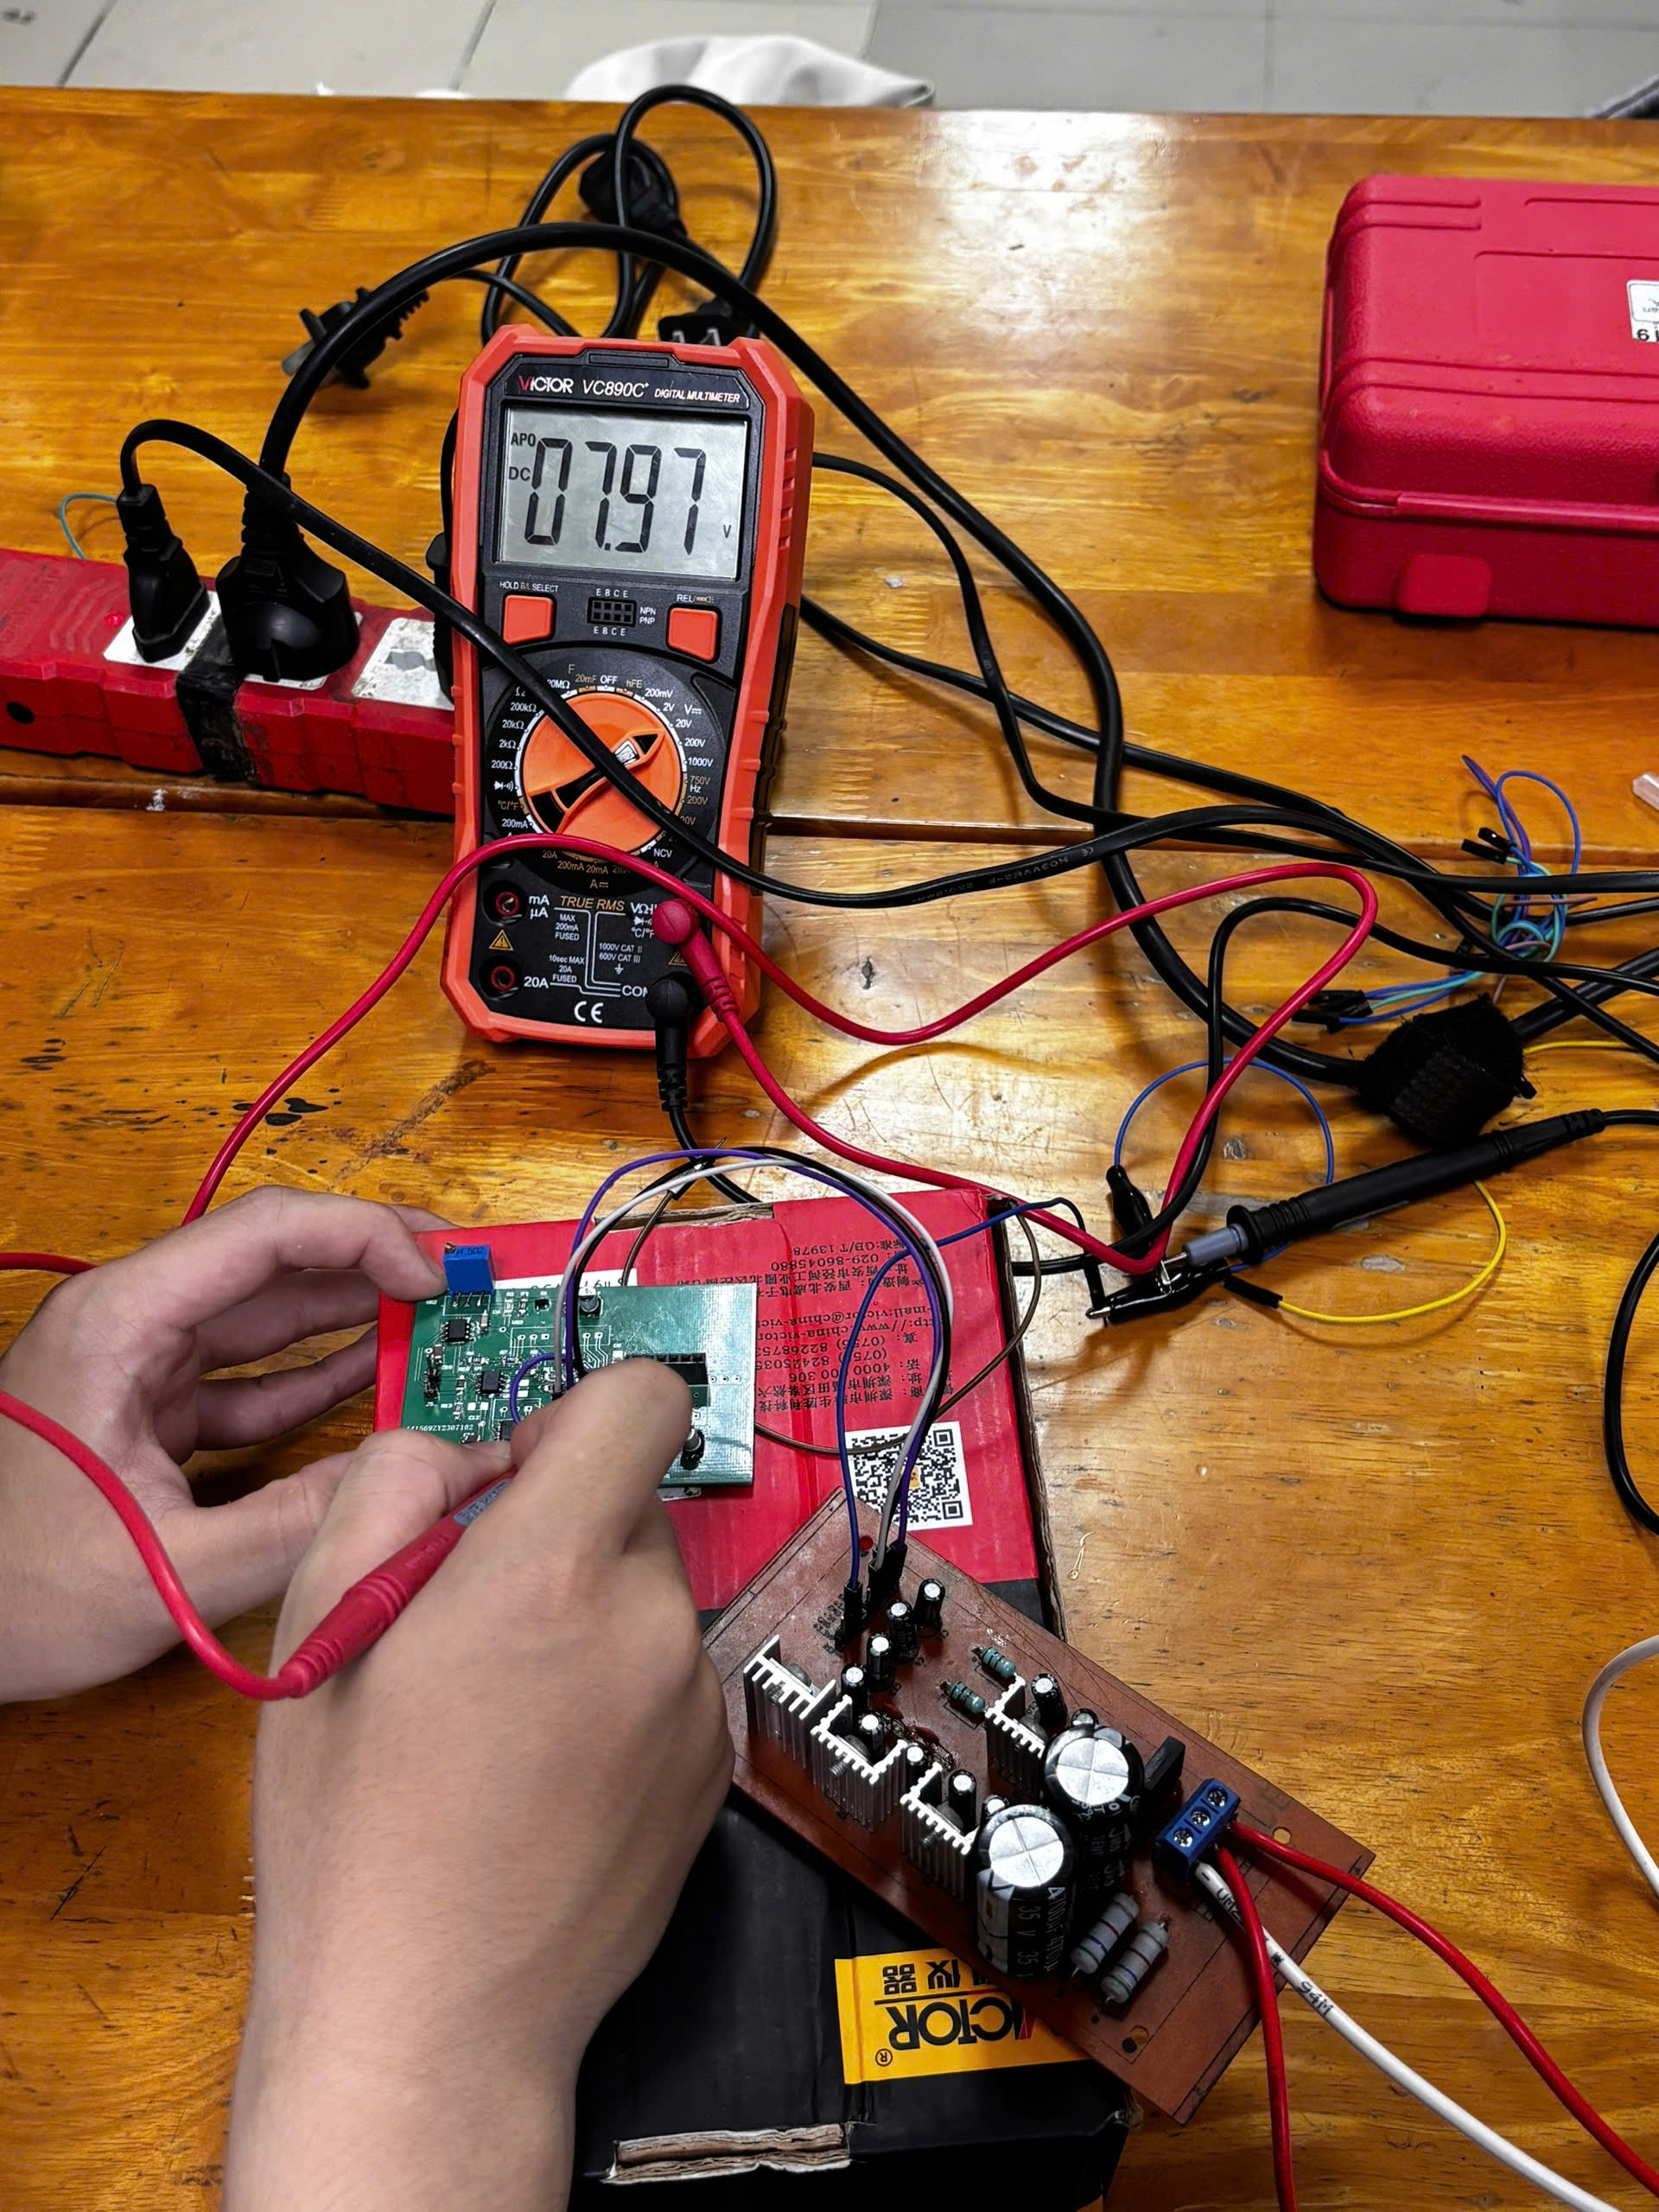
\includegraphics[width=0.7\linewidth]{my-chapters/my-images/Circuit_sim/CIRCUIT_8V}
	\caption{Kiểm tra mạch tạo điên áp cộng $8\textsf{V}$.}
	\label{fig:circuit8v}
\end{figure}

\begin{figure}[H]
	\centering
	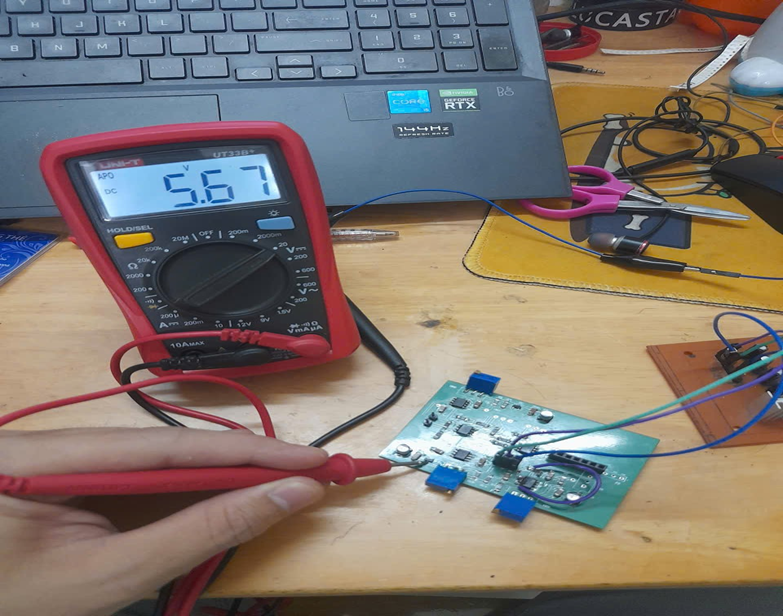
\includegraphics[width=0.7\linewidth]{my-chapters/my-images/Circuit_sim/CIRCUIT_check_zenor}
	\caption{Kiểm tra điện áp Zenner.}
	\label{fig:circuitcheckzenor}
\end{figure}

Nhóm tiến hành đo đạc lần 1 và 2 và kết quả thu được khi chưa calibre mạch (video khảo sát lần 1 :\href{https://youtu.be/ByMETPjAgkQ}{thislink}) ; (video khảo sát lần 2 : \href{https://youtu.be/FqDw9E245dE}{thislink})

\begin{table}[H]
	\centering
	\caption{Bảng số liệu đo đạc điện áp theo nhiệt độ}
	\vspace{0.2cm}
	\begin{tabular}{|c|c|c|}
		\hline
		\textbf{Nhiệt độ} & \textbf{Lần 1 (V)} & \textbf{Lần 2 (V)} \\
		\hline
		15$^\circ$C & 0.45 & 0.42 \\
		\hline
		20$^\circ$C & 0.72 & 0.57 \\
		\hline
		25$^\circ$C & 0.88 & 0.88 \\
		\hline
		30$^\circ$C & 1.16 & 1.13 \\
		\hline
		35$^\circ$C & 1.4 & 1.09 \\
		\hline
		40$^\circ$C & 1.72 & 1.84 \\
		\hline
		45$^\circ$C & 2.03 & 2.17 \\
		\hline
		50$^\circ$C & 2.38 & 2.43 \\
		\hline
		55$^\circ$C & 2.77 & 2.75 \\
		\hline
		60$^\circ$C & 3.13 & 3.08 \\
		\hline
		65$^\circ$C & 3.51 & 3.77 \\
		\hline
		70$^\circ$C & 5.7 & 9.16 \\
		\hline
		75$^\circ$C & 9.29 & 8.9 \\
		\hline
		80$^\circ$C & 9.16 & 8.67 \\
		\hline
	\end{tabular}
\end{table}

\begin{itemize}
	\item \textbf{Nhận xét:} Điện áp có xu hướng tăng theo nhiệt độ nhưng từ khoảng 65 độ trở đi điện áp đạt tới 8 đến 9V.
\end{itemize}

Nhóm tiến hành calibre mạch đầu tiên nhóm đo điện trở ban đầu của NTC và kết quả đo là $8.08 \, k\Omega$ từ phương trình trong datasheet ta có:

\[
\text{Với } Ref = 10k, \quad T = 303.7 \, K, \quad t = 30 (^\circ C)
\]

Nhưng khi đo đạc điện áp ở ngõ ra ban đầu là $1.5V$ điều này cho thấy sự sai lệch khá lớn với lý thuyết khi tại $30 (^\circ C)$ điện áp tại ngõ ra sẽ khoảng $0.738 \, V$, độ lệch khoảng $0.762 \, V$. Chính vì vậy nhóm tiến hành tinh chỉnh điện áp cộng ở ngõ ra $8V$ giảm đi một lượng xấp xỉ $0.762V$ thành $7.25 \, V$.

\begin{figure}[H]
	\centering
	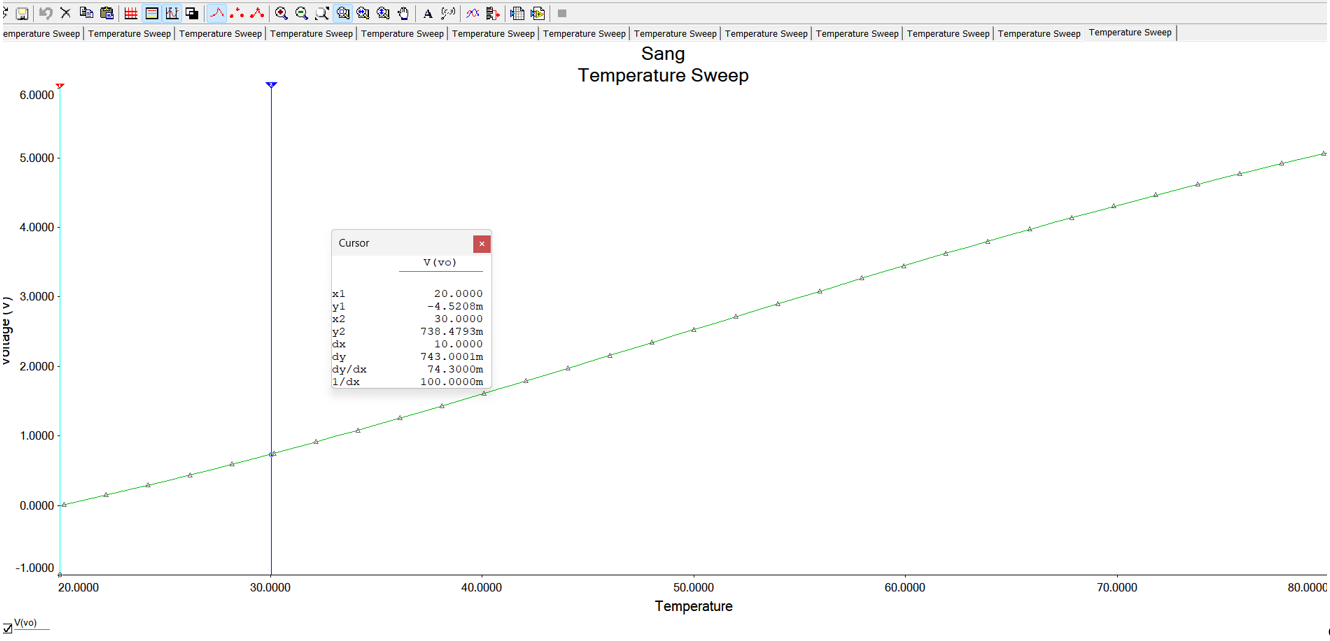
\includegraphics[width=0.9\linewidth]{my-chapters/my-images/Circuit_sim/CIRCUIT_pre_check}
	\caption{Điện áp ngõ ra tại $30^{o}C$ theo lý thuyết.}
	\label{fig:circuitprecheck}
\end{figure}

\begin{figure}[H]
	\centering
	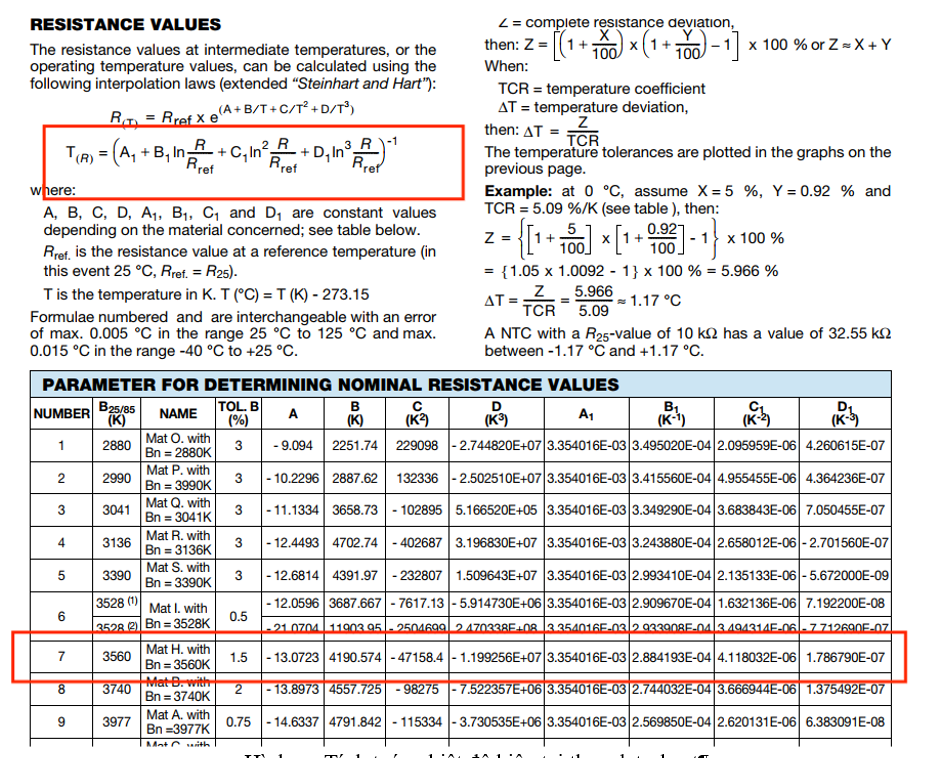
\includegraphics[width=0.9\linewidth]{my-chapters/my-images/Circuit_sim/CIRCUIT_pre_check_NTC}
	\caption{Tính toán nhiệt độ hiện tại theo datasheet.}
	\label{fig:circuitprecheckntc}
\end{figure}

\begin{figure}[H]
	\centering
	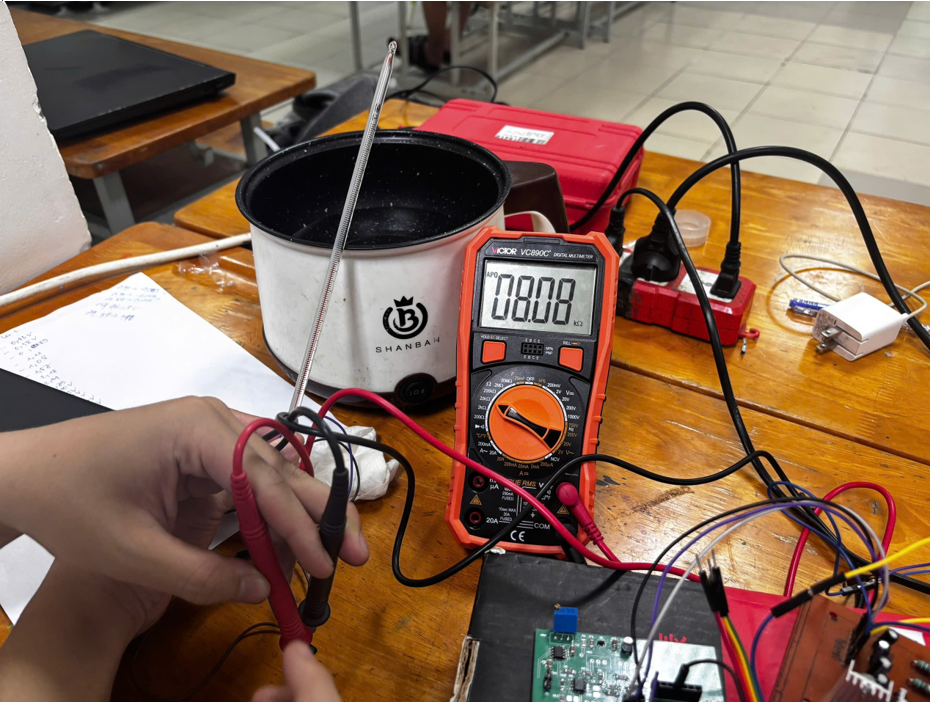
\includegraphics[width=0.8\linewidth]{my-chapters/my-images/Circuit_sim/CIRCUIT_pre_check_NTC_Vol}
	\caption{Kết quả đo điện trở ban đầu của NTC.}
	\label{fig:circuitprecheckntcvol}
\end{figure}

\begin{figure}[H]
	\centering
	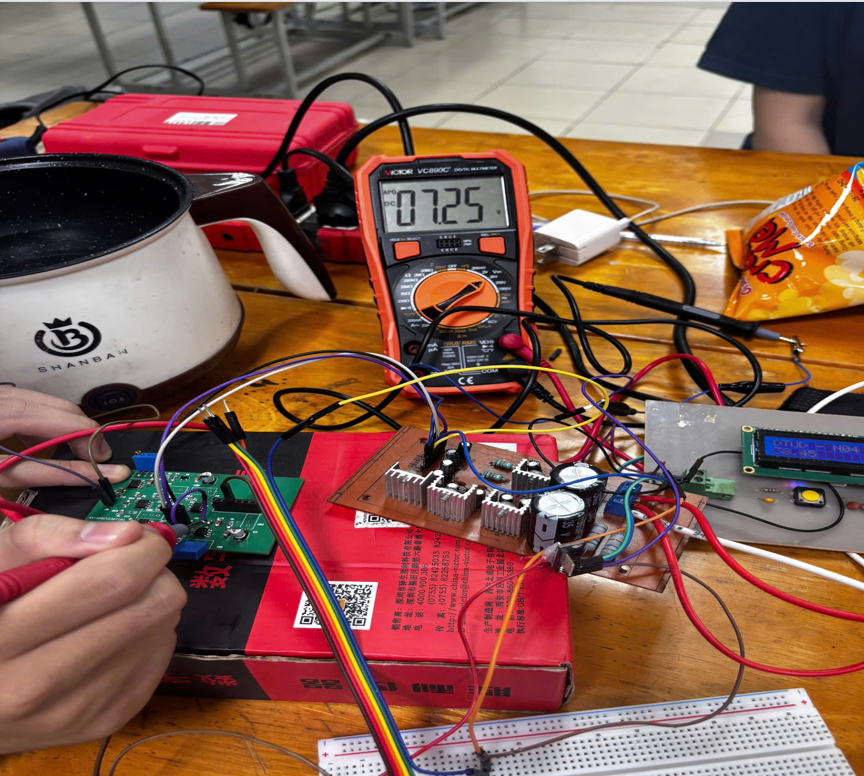
\includegraphics[width=0.8\linewidth]{my-chapters/my-images/Circuit_sim/CIRCUIT_pre_check_NTC_After_Vol}
	\caption{Tinh chỉnh điện áp từ $8\textsf{V}$ xuống $7.25\textsf{V}$.}
	\label{fig:circuitprecheckntcaftervol}
\end{figure}

Sau đó nhóm tiến hành khảo sát nhiệt độ và được kết quả thực nghiệm (video khảo sát : \href{https://youtu.be/sqnxJhxf1RI}{thislink})

%\begin{table}[H]
%	\centering
%	\caption{Kết quả thực nghiệm khảo sát nhiệt độ và điện áp}
%	\vspace{0.2cm}
%	\begin{tabular}{|c|c|}
%		\hline
%		\textbf{Nhiệt độ} & \textbf{Điện áp (V)} \\
%		\hline
%		15$^\circ$C & -0.12 \\
%		\hline
%		20$^\circ$C & 0.08 \\
%		\hline
%		25$^\circ$C & 0.39 \\
%		\hline
%		30$^\circ$C & 0.76 \\
%		\hline
%		35$^\circ$C & 1.13 \\
%		\hline
%		40$^\circ$C & 1.53 \\
%		\hline
%		45$^\circ$C & 2.08 \\
%		\hline
%		50$^\circ$C & 2.35 \\
%		\hline
%		55$^\circ$C & 2.69 \\
%		\hline
%		60$^\circ$C & 3.82 \\
%		\hline
%		65$^\circ$C & 5.92 \\
%		\hline
%		70$^\circ$C & 5.92 \\
%		\hline
%		75$^\circ$C & 5.92 \\
%		\hline
%		80$^\circ$C & 5.92 \\
%		\hline
%	\end{tabular}
%\end{table}

\begin{figure}[H]
	\centering
	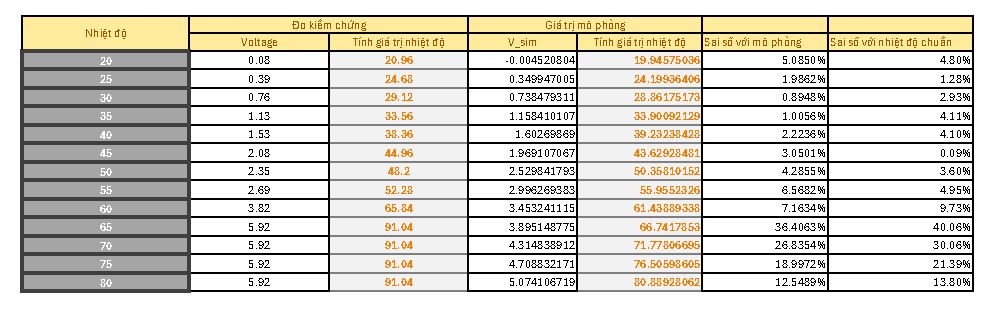
\includegraphics[width=\linewidth]{./my-ref/saiso_dodac.pdf}
	\caption{Kết quả thực nghiệm khảo sát nhiệt độ và điện áp.}
\end{figure}

\begin{itemize}
	\item \textbf{Nhận xét:} Từ nhiệt độ $20 \rightarrow 80 ^{o}C$ mach dao động từ 0.08 V đến 5.92V và từ 65 độ trở đi hầu như điện áp luôn bị ghim ở khoản $5.92\textsf{V}$.
\end{itemize}

Để biết được lý do việt từ 65 độ trở đi điện áp luôn bị ghim ở 5.92 V nhóm tiến hành khảo sát điện áp ngõ vào của INA128 vào ngõ ra ( video khảo sát \href{https://youtu.be/FasT7o_97dM}{thislink})

Từ video khảo sát ta có thấy từ khoảng 65 độ trở đi sự thay đổi điện áp ngõ vào gần như chỉ khoảng từ vài mV điều này khiến cho vôn kế không thể thay đổi nên điện áp luôn hiện thị $5.92$ đến $5.94\textsf{V}$.

\subsubsection{Kết luận}

Về cơ bản, mạch đã hoạt động đúng theo yêu cầu thiết kế ban đầu: khi nhiệt độ môi trường tăng, điện áp ngõ ra cũng tăng tương ứng. Tuy nhiên, kết quả thu được vẫn tồn tại sự sai số khá lớn so với tính toán lý thuyết. Những nguyên nhân chính dẫn đến sự sai lệch này có thể xuất phát từ dung sai của linh kiện, phương pháp đo đạc thủ công chưa đồng bộ, hoặc do ảnh hưởng của nhiễu từ môi trường xung quanh.
Bên cạnh vấn đề về sai số, trong quá trình thực hiện đề tài nhóm cũng đã đối mặt với không ít khó khăn. Việc tính toán để tuyến tính hóa đặc tuyến của cảm biến NTC cũng như cân chỉnh mạch sao cho hoạt động ổn định đòi hỏi nhiều thời gian thử nghiệm và khắc phục lỗi.

Mặc dù vậy, kết quả đạt được ngày hôm nay là minh chứng rõ ràng cho sự nỗ lực nghiên cứu và tinh thần làm việc nghiêm túc của tập thể nhóm.  Đề tài này không chỉ giúp nhóm hoàn thành mục tiêu học tập mà còn mang lại những kinh nghiệm thực tiễn quý báu .

\section{Thực hiện mạch nguồn}

\begin{figure}[H]
	\centering
	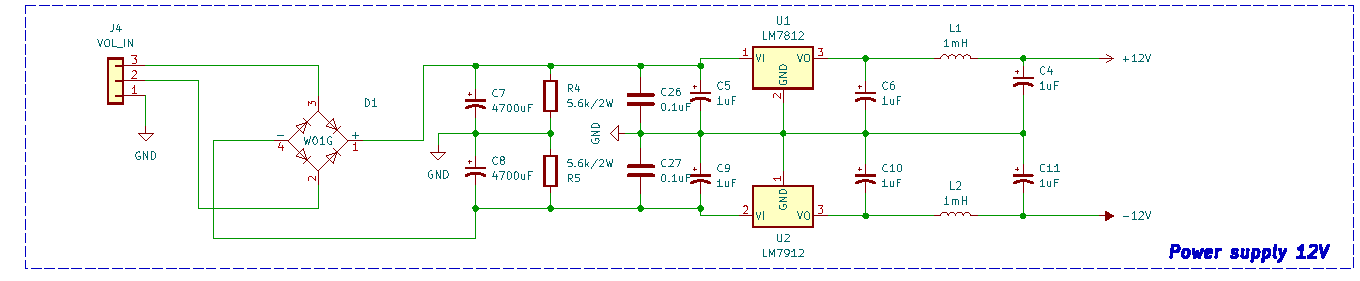
\includegraphics[width=.9\linewidth]{./my-chapters/my-images/Power_Source/power_supply.pdf}
	\caption{Tổng quan của mạch nguồn.}
\end{figure}

\subsection{Điện áp sau khi chỉnh lưu}

\begin{figure}[H]
	\centering
	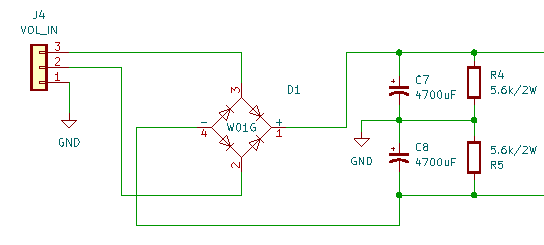
\includegraphics[width=0.6\linewidth]{./my-chapters/my-images/Power_Source/mach_chinh_luu.pdf}
	\caption{Mạch chỉnh lưu điện áp đầu vào.}
	\label{f_mach chinh luu}
\end{figure}

Giá trị VOL\_IN được cấp bởi đầu ra của biến áp với điện áp đầu ra của biến áp là $12VAC$, sau khi chỉnh lưu toàn sóng với tụ lọc là $C_7$ và $C_8$ thì điện áp ngõ ra của cầu diode được tính toán bằng công thức: \[V_{DC} = \sqrt{2}\times V_{AC} - 2\times V_{diode} \approx 15.6V\]
Trong đó, 
\begin{itemize}[label=-]
	\item $V_{DC}$: là điện áp ngõ ra sau khi chỉnh lưu toán sóng ($V$).
	\item $V_{AC}$: là điện áp ngõ vào cầu diode ($=12V$).
	\item $V_{diode}$: là sụt áp trên hai diode trong cầu chỉnh lưu ($=0.7V$).
\end{itemize}

Tụ $C_{7}$ và $C_{8}$ có chức năng làm giảm độ gợn sóng (ripple) và được tính bằng công thức: \[C = \dfrac{I}{f \times \Delta V} = 5000\mu F \approx 4700\mu F\]
Trong đó,
\begin{itemize}[label = -]
	\item $C$: là giá trị điện dung của tụ ($F$).
	\item $I$: là giá trị dòng tổng ($=1A$).
	\item $f$: là giá trị tần số sau khi chỉnh lưu ($=100Hz$).
	\item $\Delta V$: là độ gợn sóng mong muốn ($=2V$).
\end{itemize}

Điện trở $R_{4}$ và $R_{5}$ được gọi là \textit{Bleeder resistor} có tác dụng xả điện áp ở tụ $C_{7}$ và $C_{8}$ khi ngắt nguồn điện để đảm bảo an toàn cho hệ thống trong những trường hợp nguy hiểm xảy ra gây cho hai tụ này luôn nạp trong thời gian dài. Điện trở này sẽ có giá trị từ $2.2 \sim 10k\Omega$ và công suất từ $2 \sim 10W$.

\subsection{Điện áp cấp $+12V$}

\begin{figure}[H]
	\centering
	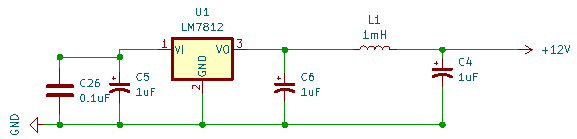
\includegraphics[width=0.6\linewidth]{./my-chapters/my-images/Power_Source/supply_+12V.pdf}
	\caption{Mạch cung cấp nguồn $+12V$.}
	\label{f_powersupply_+12V}
\end{figure}

Điện áp ngõ vào ($V_{in}$) của mạch cần phải đáp ứng tối thiểu theo công thức: \[ V_{in} > V_{out} + V_{dropout} = 12 + 2 = 14V \rightarrow V_{in} > 14V\]
Trong đó,
\begin{itemize}[label = -]
	\item $V_{in}$: là điện áp đầu vào ($V$).
	\item $V_{out}$: là điện áp đầu ra của LM7812 $=12V$.
	\item $V_{dropout}$: là điện áp rơi trên LM7812 $=2V$.
\end{itemize}

Công suất tiêu tán ($P_{loss}$) là công suất tiêu hao năng lượng dưới dạng nhiệt khi ổn áp: \[ P_{loss} = (V_{in} - V_{out}) \times I_{load} = (15.6 - 12)\times 1 = 3.6W\]
Trong đó,
\begin{itemize}[label=-]
	\item $P_{loss}$: là công suất tiêu tán trên LM7812 ($W$).
	\item $V_{in}$: là điện áp ngõ vào LM7812 ($=15.6V$).
	\item $V_{out}$: là điện áp ngõ ra LM7812 ($=12$).
	\item $I_{load}$: là dòng tải ($=1A$).
\end{itemize}

Kích thước tản nhiệt ($R_{th}$) để đảm bảo IC không quá nóng, nhiệt độ $T_j$ phải nằm trong giới hạn ($T_j \leq 125^{\circ}C$). Ta sử dụng công thức: \[ T_{j} = T_{o} + P_{loss} \times R_{th(tot)} \rightarrow R_{th(tot)} \leq \dfrac{T_{j} - T_{o}}{P_{loss}} = \dfrac{125 - 25}{3.6} \approx 27.8 \rightarrow R_{th(tot)} \leq 27.8^{\circ}C/W
\]
\[ \Rightarrow R_{th(c-a)} \leq R_{th(tot)} - R_{th(j-c)} = 27.8 - 5 \rightarrow R_{th(c-a)} \leq 22.8^{\circ}C/W \]
Trong đó,
\begin{itemize}[label = -]
	\item $T_{j}$: là nhiệt độ cho phép hoạt động của IC ($ ^\circ C$).
	\item $T_{o}$: là nhiệt độ của môi trường ($=25^{\circ}C$).
	\item $P_{loss}$: là công suất tiêu tán trên LM7812 ($=3.6W$).
	\item $R_{th(tot)}$: là tổng trở nhiệt từ junction đến môi trường ($27.8^{\circ}C/W$).
	\item $R_{th(j-c)}$: là trở nhiệt junction-to-case ($=5^{\circ}C/W$).
	\item $R_{th(c-a)}$: là trở nhiệt case-to-air ($^{\circ}C/W$).
\end{itemize}

Tụ điện đầu vào $C_{5}$ giúp bù sụt áp tạm thời và có giá trị là $1\mu F$.

Tụ điện đầu ra $C_{4}$ và $C_6$ giúp cải thiện ổn định điện áp đầu ra và có giá trị là $1\mu F$.

Tụ $C_{26}$ là tụ điện có chức năng dập nhiễu cao tần có giá trị là $0.1\mu F$.

Cuộn cảm $L_{1}$ có chức năng loại bỏ các nhiễu tần số cao có thể xuất hiện đầu ra, và tạo thành một bộ lọc LC giúp làm mịn điện áp đầu ra bằng cách giảm biên độ của các gợn sóng còn lại sau khi chỉnh lưu và ổn áp.

Hiệu suất ($\eta$) của mạch được tính bằng công thức: \[ \eta = \dfrac{V_{out}\times I_{load}}{V_{in} \times I_{load}}\times 100\% = \dfrac{12\times 1}{15.6 \times 1}\times 100\% \approx 76.9\% \]

\subsection{Điện áp cấp $-12V$}

\begin{figure}[H]
	\centering
	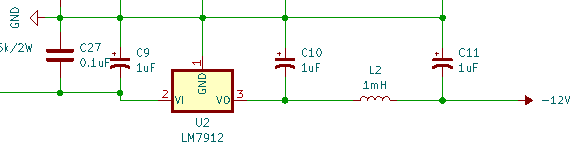
\includegraphics[width=0.6\linewidth]{./my-chapters/my-images/Power_Source/supply_-12V.pdf}
	\caption{Mạch cung cấp nguồn $-12V$.}
	\label{f_powersupply_-12V}
\end{figure}

Điện áp ngõ vào ($V_{in}$) của mạch cần phải đáp ứng tối thiểu theo công thức: \[ V_{in} < V_{out} - V_{dropout} = -12 - 2 = -14V \rightarrow V_{in} < -14V\]
Trong đó,
\begin{itemize}[label = -]
	\item $V_{in}$: là điện áp đầu vào ($V$).
	\item $V_{out}$: là điện áp đầu ra của LM7912 $=-12V$.
	\item $V_{dropout}$: là điện áp rơi trên LM7912 $=2V$.
\end{itemize}

Công suất tiêu tán ($P_{loss}$) là công suất tiêu hao năng lượng dưới dạng nhiệt khi ổn áp: \[ P_{loss} = (|V_{in}| - |V_{out}|) \times I_{load} = (15.6 - 12)\times 1 = 3.6W\]
Trong đó,
\begin{itemize}[label=-]
	\item $P_{loss}$: là công suất tiêu tán trên LM7912 ($W$).
	\item $V_{in}$: là điện áp ngõ vào LM7912 ($=-15.6V$).
	\item $V_{out}$: là điện áp ngõ ra LM7912 ($=-12$).
	\item $I_{load}$: là dòng tải ($=1A$).
\end{itemize}

Kích thước tản nhiệt ($R_{th}$) để đảm bảo IC không quá nóng, nhiệt độ $T_j$ phải nằm trong giới hạn ($T_j \leq 125^{\circ}C$). Ta sử dụng công thức: \[ T_{j} = T_{o} + P_{loss} \times R_{th(tot)} \rightarrow R_{th(tot)} \leq \dfrac{T_{j} - T_{o}}{P_{loss}} = \dfrac{125 - 25}{3.6} \approx 27.8 \rightarrow R_{th(tot)} \leq 27.8^{\circ}C/W
\]
\[ \Rightarrow R_{th(c-a)} \leq R_{th(tot)} - R_{th(j-c)} = 27.8 - 5 \rightarrow R_{th(c-a)} \leq 22.8^{\circ}C/W \]
Trong đó,
\begin{itemize}[label = -]
	\item $T_{j}$: là nhiệt độ cho phép hoạt động của IC ($ ^\circ C$).
	\item $T_{o}$: là nhiệt độ của môi trường ($=25^{\circ}C$).
	\item $P_{loss}$: là công suất tiêu tán trên LM7912 ($=3.6W$).
	\item $R_{th(tot)}$: là tổng trở nhiệt từ junction đến môi trường ($27.8^{\circ}C/W$).
	\item $R_{th(j-c)}$: là trở nhiệt junction-to-case ($=5^{\circ}C/W$).
	\item $R_{th(c-a)}$: là trở nhiệt case-to-air ($^{\circ}C/W$).
\end{itemize}

Tụ điện đầu vào $C_{9}$ giúp bù sụt áp tạm thời và có giá trị là $1\mu F$.

Tụ điện đầu ra $C_{10}$ và $C_{11}$ giúp cải thiện ổn định điện áp đầu ra và có giá trị là $1\mu F$.

Tụ $C_{27}$ là tụ điện có chức năng dập nhiễu cao tần có giá trị là $0.1\mu F$.

Cuộn cảm $L_{2}$ có chức năng loại bỏ các nhiễu tần số cao có thể xuất hiện đầu ra, và tạo thành một bộ lọc LC giúp làm mịn điện áp đầu ra bằng cách giảm biên độ của các gợn sóng còn lại sau khi chỉnh lưu và ổn áp.

Hiệu suất ($\eta$) của mạch được tính bằng công thức: \[ \eta = \dfrac{V_{out}\times I_{load}}{V_{in} \times I_{load}}\times 100\% = \dfrac{12\times 1}{15.6 \times 1}\times 100\% \approx 76.9\% \]

\subsection{Điện áp cấp $+5V$}

\begin{figure}[H]
	\centering
	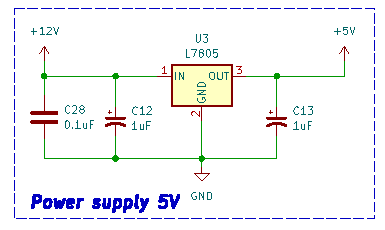
\includegraphics[width=0.6\linewidth]{./my-chapters/my-images/Power_Source/power_supply_5V.pdf}
	\caption{Mạch cung cấp nguồn $+5V$}
	\label{f_supply_+5V}
\end{figure}

Điện áp ngõ vào ($V_{in}$) của mạch cần phải đáp ứng tối thiểu theo công thức: \[ V_{in} > V_{out} + V_{dropout} = 5 + 2 = 7V \rightarrow V_{in} > 7V\]
Trong đó,
\begin{itemize}[label = -]
	\item $V_{in}$: là điện áp đầu vào ($V$).
	\item $V_{out}$: là điện áp đầu ra của LM7805 $=5V$.
	\item $V_{dropout}$: là điện áp rơi trên LM7805 $=2V$.
\end{itemize}

Công suất tiêu tán ($P_{loss}$) là công suất tiêu hao năng lượng dưới dạng nhiệt khi ổn áp: \[ P_{loss} = (V_{in} - V_{out}) \times I_{load} = (12 - 5)\times 1 = 7W\]
Trong đó,
\begin{itemize}[label=-]
	\item $P_{loss}$: là công suất tiêu tán trên LM7805 ($W$).
	\item $V_{in}$: là điện áp ngõ vào LM7805 ($=12V$).
	\item $V_{out}$: là điện áp ngõ ra LM7805 ($=5V$).
	\item $I_{load}$: là dòng tải ($=1A$).
\end{itemize}

Kích thước tản nhiệt ($R_{th}$) để đảm bảo IC không quá nóng, nhiệt độ $T_j$ phải nằm trong giới hạn ($T_j \leq 125^{\circ}C$). Ta sử dụng công thức: \[ T_{j} = T_{o} + P_{loss} \times R_{th(tot)} \rightarrow R_{th(tot)} \leq \dfrac{T_{j} - T_{o}}{P_{loss}} = \dfrac{125 - 25}{7} \approx 14.3 \rightarrow R_{th(tot)} \leq 14.3^{\circ}C/W
\]
\[ \Rightarrow R_{th(c-a)} \leq R_{th(tot)} - R_{th(j-c)} = 14.3 - 5 \rightarrow R_{th(c-a)} \leq 9.3^{\circ}C/W \]
Trong đó,
\begin{itemize}[label = -]
	\item $T_{j}$: là nhiệt độ cho phép hoạt động của IC ($ ^\circ C$).
	\item $T_{o}$: là nhiệt độ của môi trường ($=25^{\circ}C$).
	\item $P_{loss}$: là công suất tiêu tán trên LM7805 ($=7W$).
	\item $R_{th(tot)}$: là tổng trở nhiệt từ junction đến môi trường ($14.3^{\circ}C/W$).
	\item $R_{th(j-c)}$: là trở nhiệt junction-to-case ($=5^{\circ}C/W$).
	\item $R_{th(c-a)}$: là trở nhiệt case-to-air ($^{\circ}C/W$).
\end{itemize}

Tụ điện đầu vào $C_{12}$ giúp bù sụt áp tạm thời và có giá trị là $1\mu F$.

Tụ điện đầu ra $C_{13}$ giúp cải thiện ổn định điện áp đầu ra và có giá trị là $1\mu F$.

Tụ $C_{28}$ là tụ điện có chức năng dập nhiễu cao tần có giá trị là $0.1\mu F$.

Hiệu suất ($\eta$) của mạch được tính bằng công thức: \[ \eta = \dfrac{V_{out}\times I_{load}}{V_{in} \times I_{load}}\times 100\% = \dfrac{5\times 1}{12 \times 1}\times 100\% \approx 41.7\% \]

%\subsection{Điện áp cấp $+3.3V$}
%
%\begin{figure}[H]
%	\centering
%	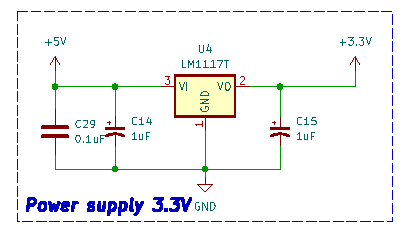
\includegraphics[width=0.6\linewidth]{./my-chapters/my-images/Power_Source/power_supply_3V.pdf}
%	\caption{Mạch cung cấp nguồn $+3.3V$}
%	\label{f_supply_+3.3V}
%\end{figure}
%
%Điện áp ngõ vào ($V_{in}$) của mạch cần phải đáp ứng tối thiểu theo công thức: \[ V_{in} > V_{out} + V_{dropout} = 3.3 + 1.2 = 4.5V \rightarrow V_{in} > 4.5V\]
%Trong đó,
%\begin{itemize}[label = -]
%	\item $V_{in}$: là điện áp đầu vào ($V$).
%	\item $V_{out}$: là điện áp đầu ra của LM117T $=3.3V$.
%	\item $V_{dropout}$: là điện áp rơi trên LM117T $=1.2V$.
%\end{itemize}
%
%Công suất tiêu tán ($P_{loss}$) là công suất tiêu hao năng lượng dưới dạng nhiệt khi ổn áp: \[ P_{loss} = (V_{in} - V_{out}) \times I_{load} = (5 - 3.3)\times 1 = 1.7W\]
%Trong đó,
%\begin{itemize}[label=-]
%	\item $P_{loss}$: là công suất tiêu tán trên LM117T ($W$).
%	\item $V_{in}$: là điện áp ngõ vào LM117T ($=5V$).
%	\item $V_{out}$: là điện áp ngõ ra LM117T ($=3.3$).
%	\item $I_{load}$: là dòng tải ($=1A$).
%\end{itemize}
%
%Kích thước tản nhiệt ($R_{th}$) để đảm bảo IC không quá nóng, nhiệt độ $T_j$ phải nằm trong giới hạn ($T_j \leq 125^{\circ}C$). Ta sử dụng công thức: \[ T_{j} = T_{o} + P_{loss} \times R_{th(tot)} \rightarrow R_{th(tot)} \leq \dfrac{T_{j} - T_{o}}{P_{loss}} = \dfrac{125 - 25}{1.7} \approx 58.8 \rightarrow R_{th(tot)} \leq 58.8^{\circ}C/W
%\]
%\[ \Rightarrow R_{th(c-a)} \leq R_{th(tot)} - R_{th(j-c)} = 58.8 - 2 \rightarrow R_{th(c-a)} \leq 56.8^{\circ}C/W \]
%Trong đó,
%\begin{itemize}[label = -]
%	\item $T_{j}$: là nhiệt độ cho phép hoạt động của IC ($ ^\circ C$).
%	\item $T_{o}$: là nhiệt độ của môi trường ($=25^{\circ}C$).
%	\item $P_{loss}$: là công suất tiêu tán trên LM117T ($=7W$).
%	\item $R_{th(tot)}$: là tổng trở nhiệt từ junction đến môi trường ($58.8^{\circ}C/W$).
%	\item $R_{th(j-c)}$: là trở nhiệt junction-to-case ($=2^{\circ}C/W$).
%	\item $R_{th(c-a)}$: là trở nhiệt case-to-air ($^{\circ}C/W$).
%\end{itemize}
%
%Tụ điện đầu vào $C_{14}$ giúp bù sụt áp tạm thời và có giá trị là $1\mu F$.
%
%Tụ điện đầu ra $C_{15}$ giúp cải thiện ổn định điện áp đầu ra và có giá trị là $1\mu F$.
%
%Tụ $C_{29}$ là tụ điện có chức năng dập nhiễu cao tần có giá trị là $0.1\mu F$.
%
%Hiệu suất ($\eta$) của mạch được tính bằng công thức: \[ \eta = \dfrac{V_{out}\times I_{load}}{V_{in} \times I_{load}}\times 100\% = \dfrac{3.3\times 1}{5 \times 1}\times 100\% = 66\% \]

\subsection{Thực thi mạch nguồn}

\begin{figure}[H]
	\centering
	\begin{minipage}{.45\linewidth}
		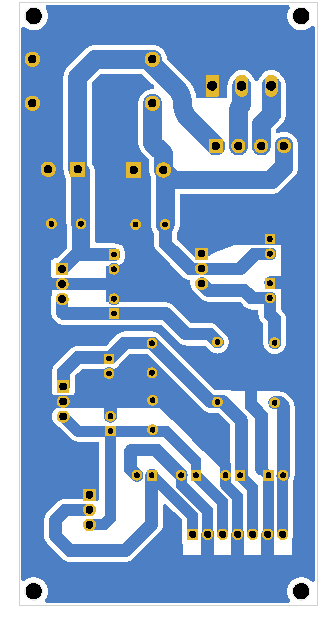
\includegraphics[width=\linewidth]{./my-chapters/my-images/Power_Source/layout_B.pdf}
	\end{minipage}
	\begin{minipage}{.45\linewidth}
		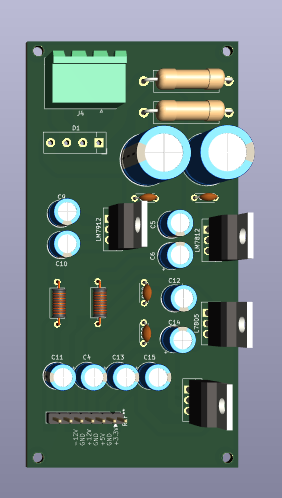
\includegraphics[width=\linewidth]{./my-chapters/my-images/Power_Source/model_3D.png}
	\end{minipage}
	\caption{Thiết kế mạch nguồn.}
\end{figure}

\begin{figure}[H]
	\centering
	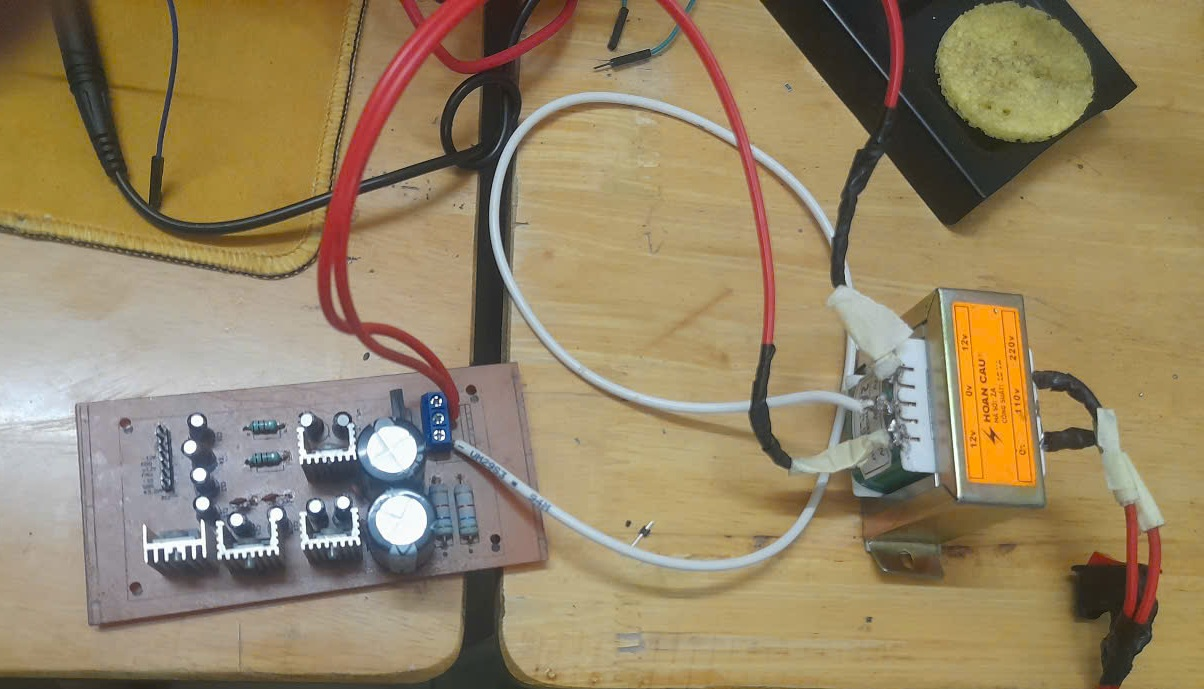
\includegraphics[width=.7\linewidth]{./my-chapters/my-images/Power_Source/mach_thucte.jpg}
	\caption{Hình ảnh thực tế của mạch nguồn.}
\end{figure}

\begin{figure}[H]
	\centering
	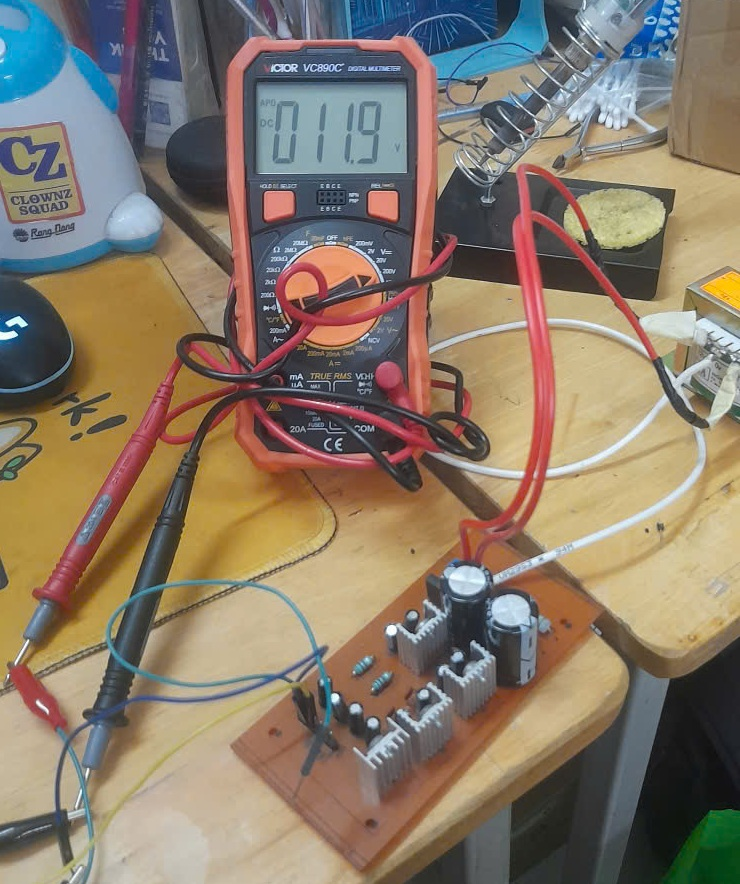
\includegraphics[width=.6\linewidth]{./my-chapters/my-images/Power_Source/thucte_+12V.jpg}
	\caption{Hình ảnh thực tế của mạch nguồn tại $+12V$.}
\end{figure}

\begin{figure}[H]
	\centering
	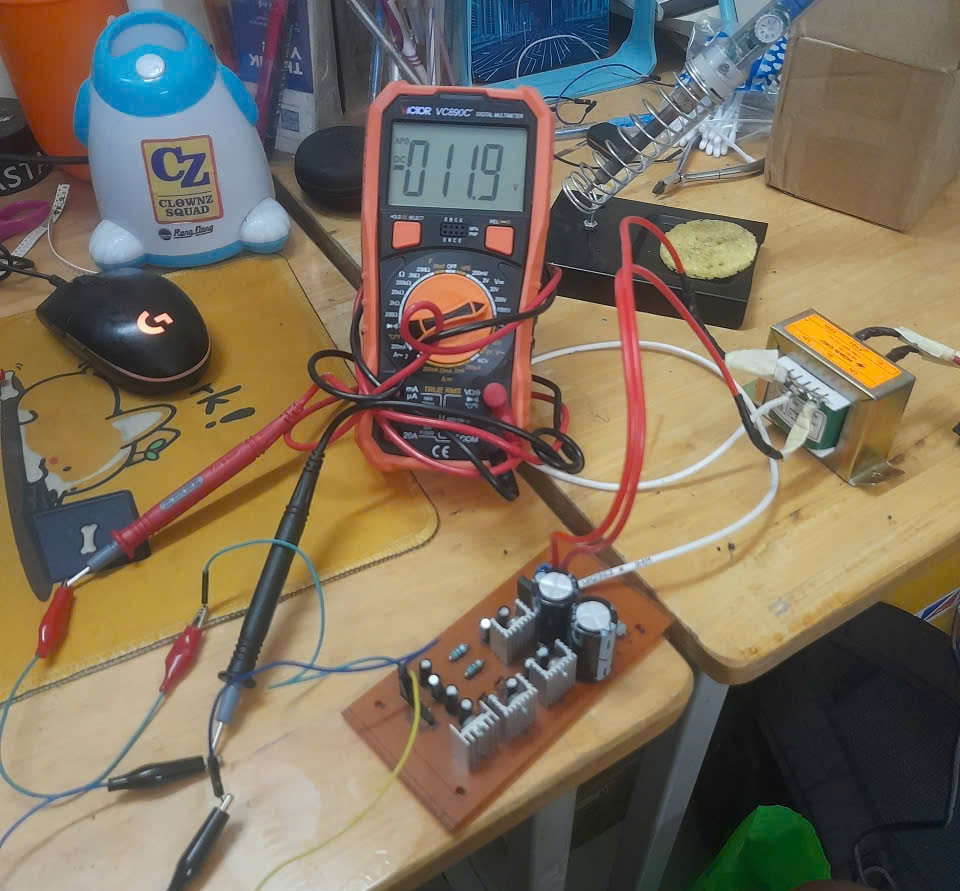
\includegraphics[width=.6\linewidth]{./my-chapters/my-images/Power_Source/thucte_-12V.jpg}
	\caption{Hình ảnh thực tế của mạch nguồn tại $-12V$.}
\end{figure}

\begin{figure}[H]
	\centering
	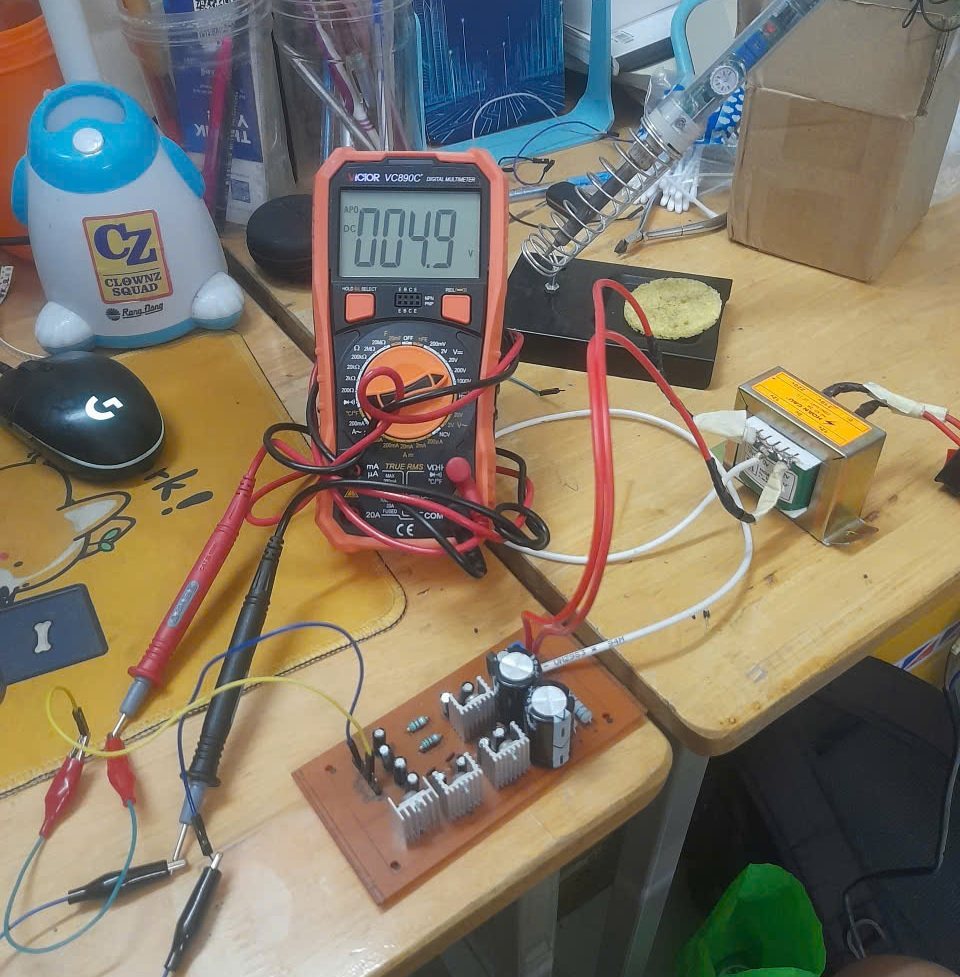
\includegraphics[width=.6\linewidth]{./my-chapters/my-images/Power_Source/thucte_5V.jpg}
	\caption{Hình ảnh thực tế của mạch nguồn tại $+5V$.}
\end{figure}
\section{Thực hiện mạch đọc ADC}

\subsection{Lưu đồ giải thuật của mạch đọc ADC}

Sử dụng ATmega328P để thực hiện xử lý dữ liệu gửi từ ADS1115 về thông qua các chân như sau:

\begin{figure}[H]
	\centering
	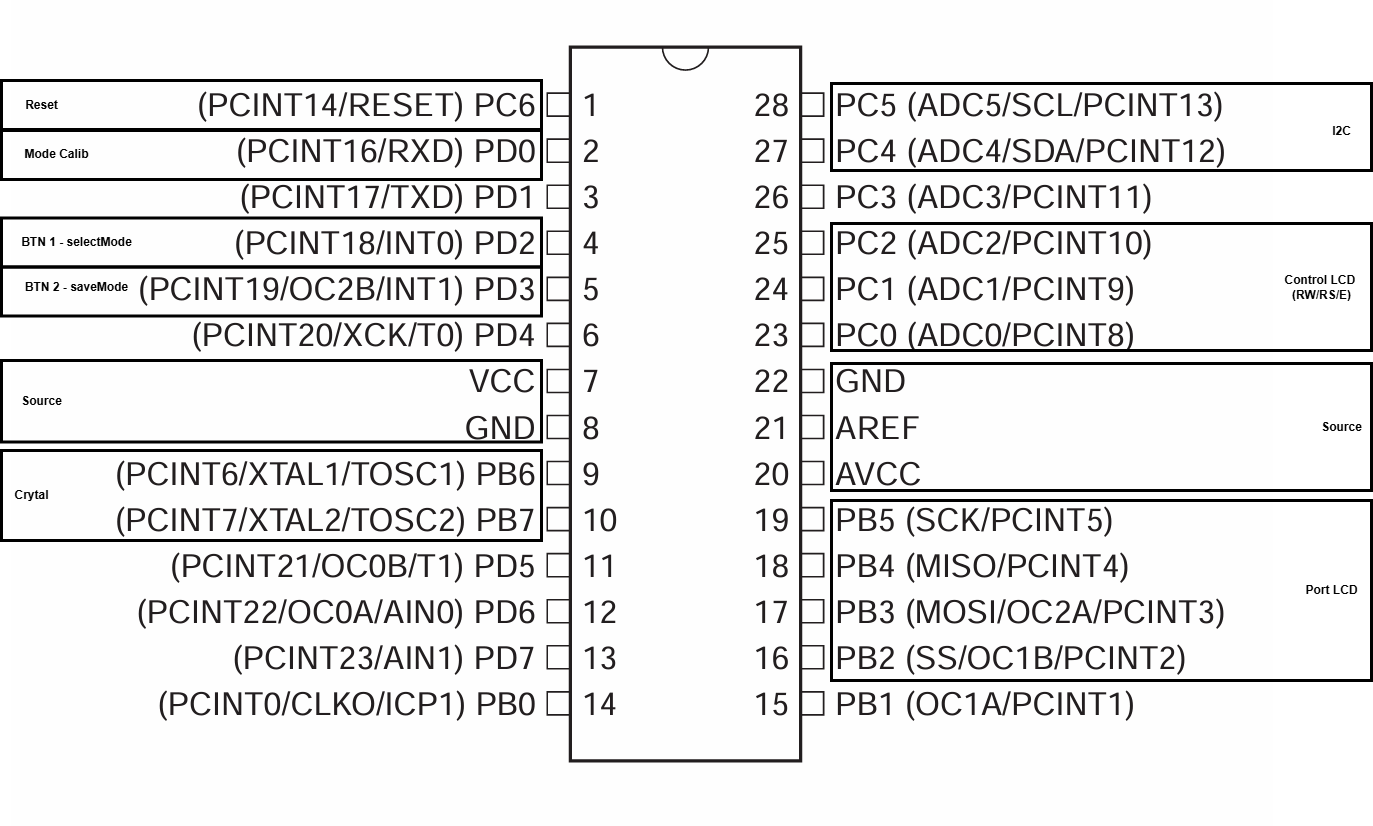
\includegraphics[width=.8\linewidth]{./my-chapters/my-images/PCB_ADC/ADC_spec_mapping.png}
	\caption{Sơ đồ kết nối chân trên ATmega328P.}
\end{figure}

\begin{figure}[H]
	\centering
	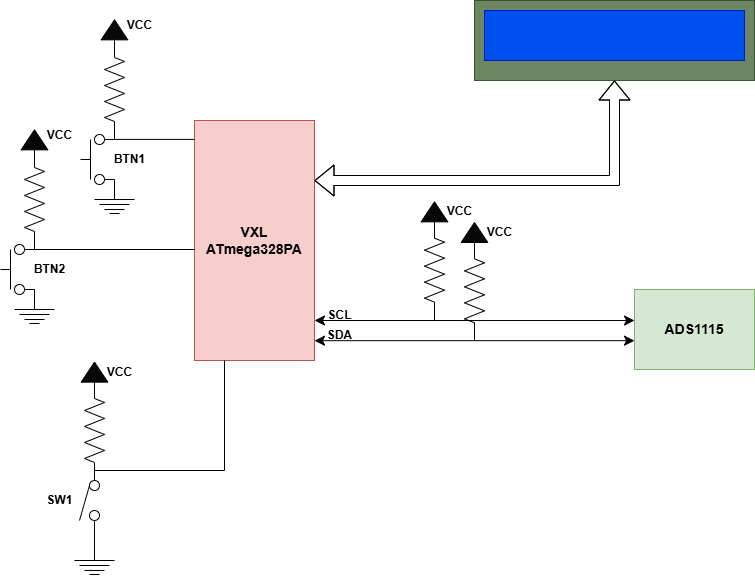
\includegraphics[width=.8\linewidth]{./my-chapters/my-images/PCB_ADC/ADC_spec_overview_connect.png}
	\caption{Sơ đồ kết nối tổng quan cho mạch đọc ADC.}
\end{figure}

\begin{figure}[H]
	\centering
	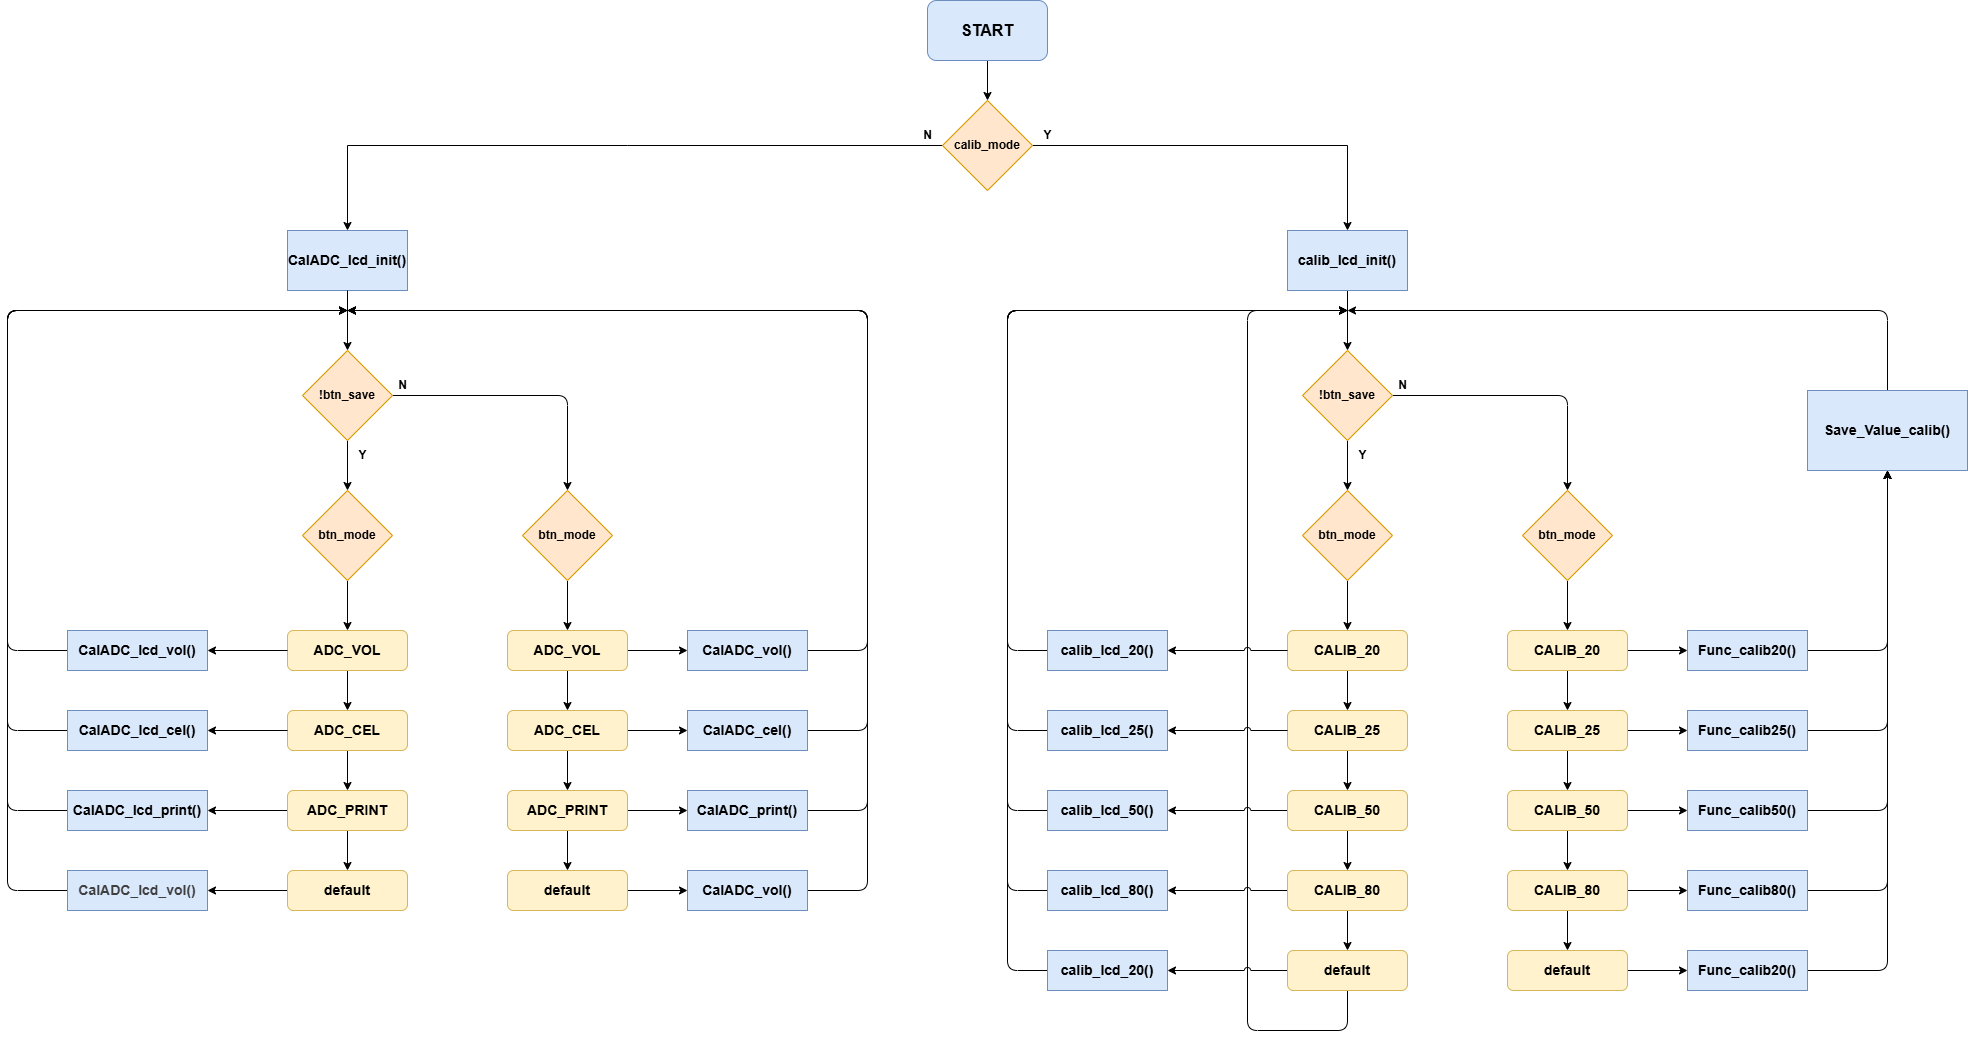
\includegraphics[width=.8\linewidth]{./my-chapters/my-images/PCB_ADC/overflow_diagram.png}
	\caption{Flowchart của mạch đo mạch ADC.}
\end{figure}

\subsection{Mạch đọc ADC}

\begin{figure}[H]
	\centering
	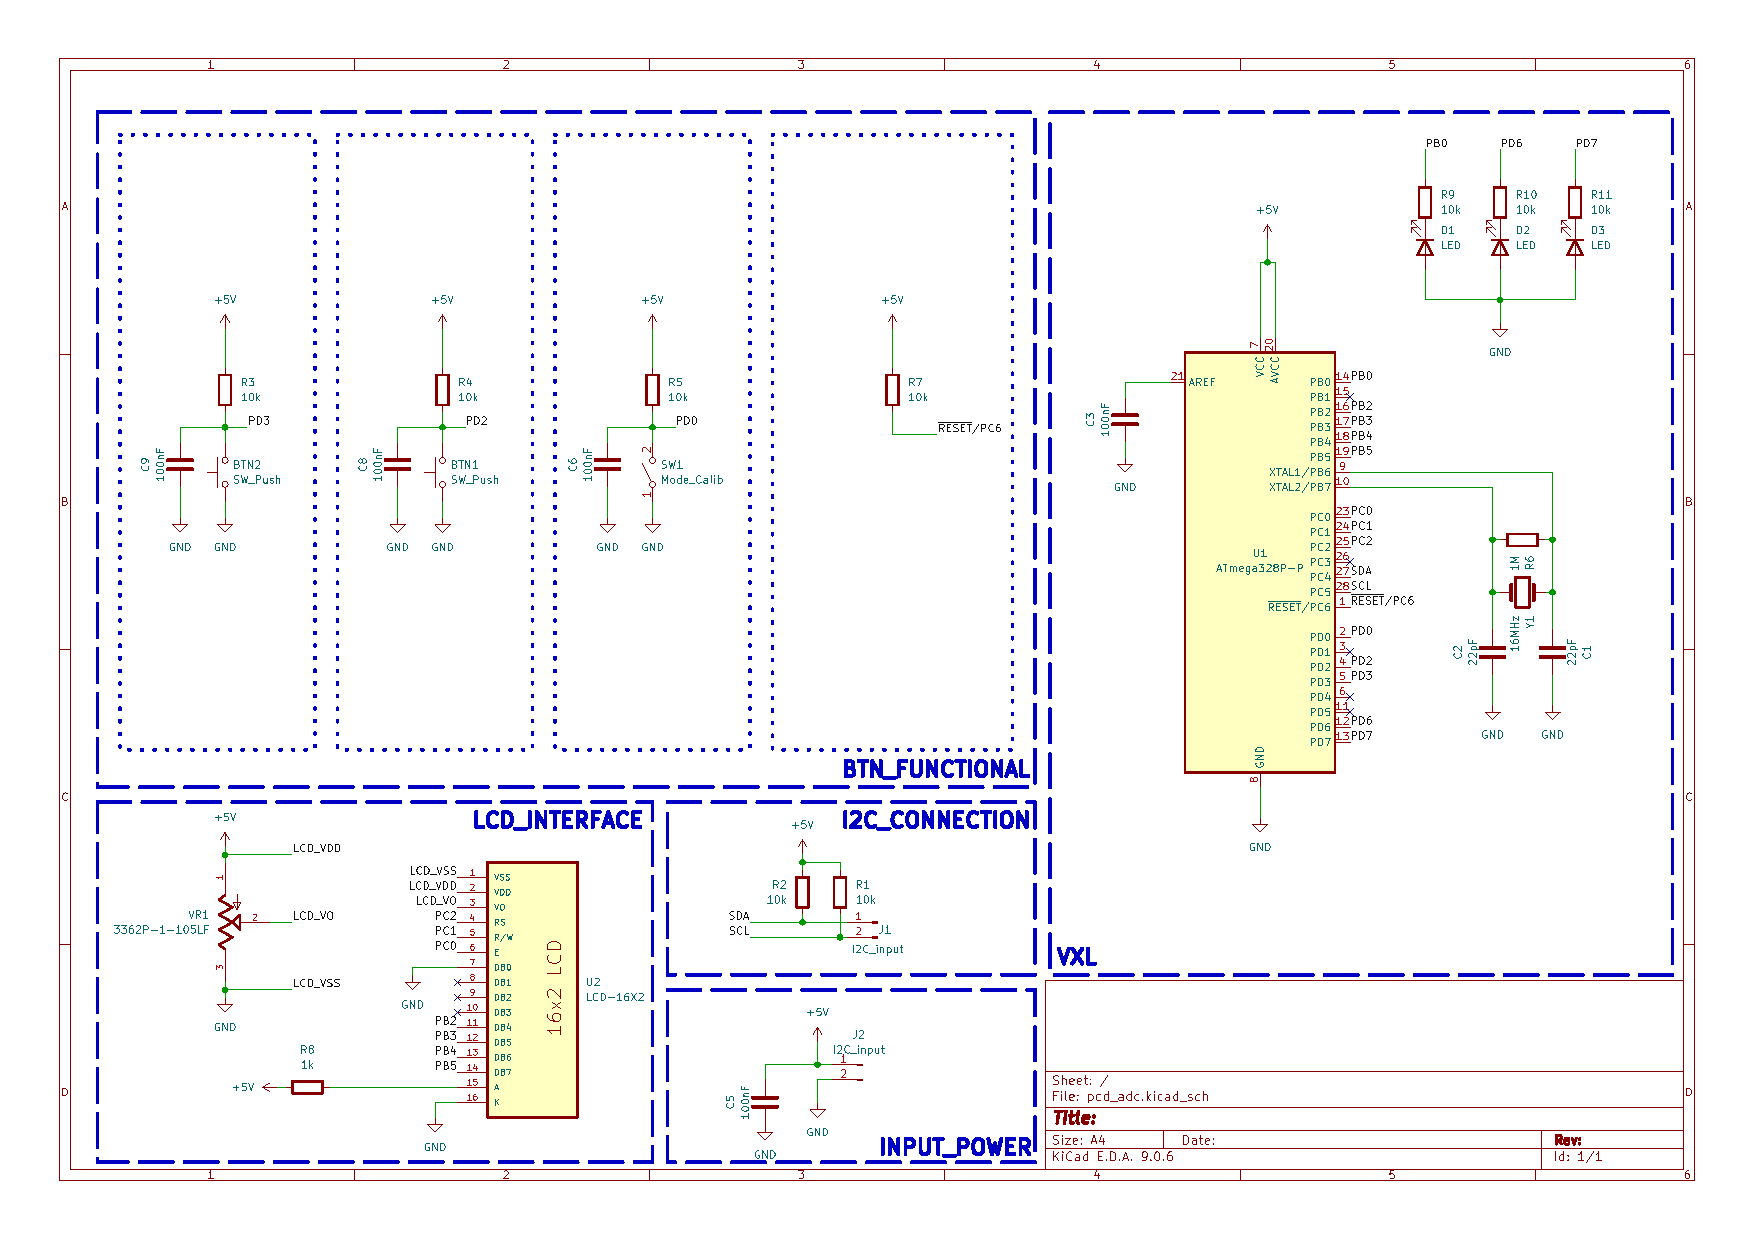
\includegraphics[width=\linewidth]{./my-chapters/my-diagrams/pcd_adc.pdf}
	\caption{Schematic của mạch đọc ADC.}
\end{figure}

\begin{figure}[H]
	\centering
	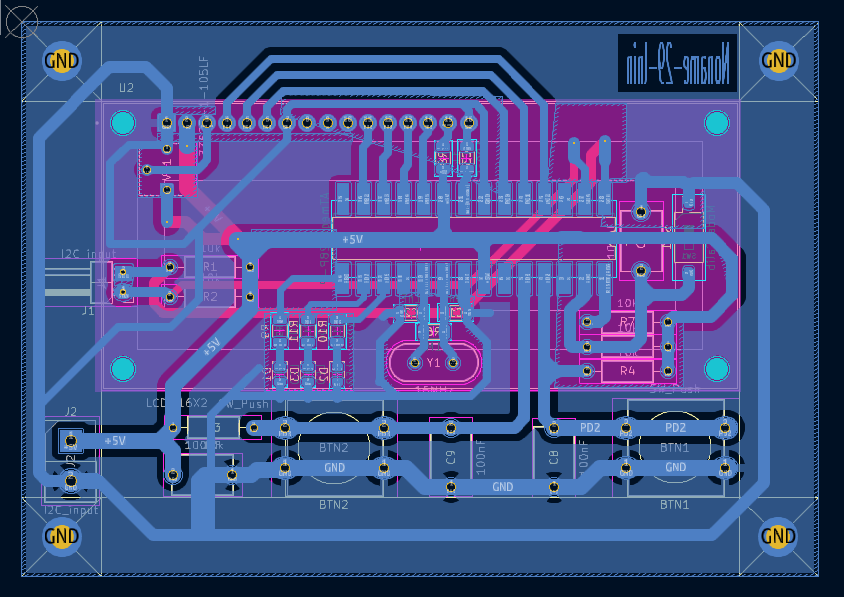
\includegraphics[width=.8\linewidth]{my-chapters/my-images/PCB_ADC/pcb_adc.png}
	\caption{Layout của mạch đọc ADC.}
\end{figure}

\begin{figure}[H]
	\centering
	\begin{minipage}{.45\linewidth}
		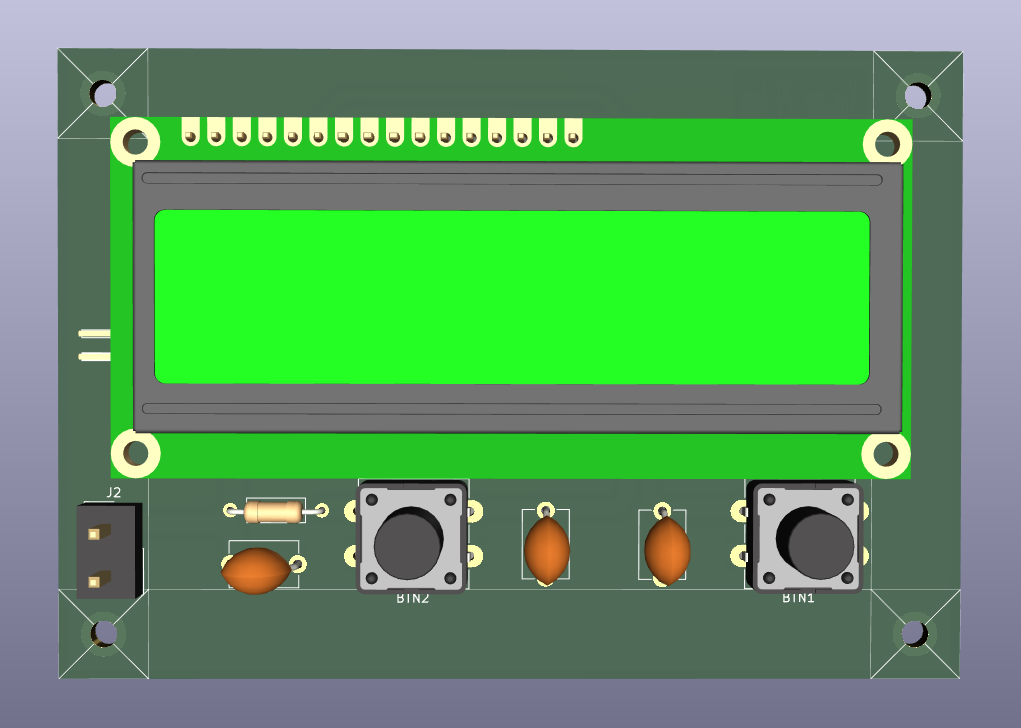
\includegraphics[width=\linewidth]{my-chapters/my-images/PCB_ADC/3D_topview.png}
	\end{minipage}
	\begin{minipage}{.45\linewidth}
		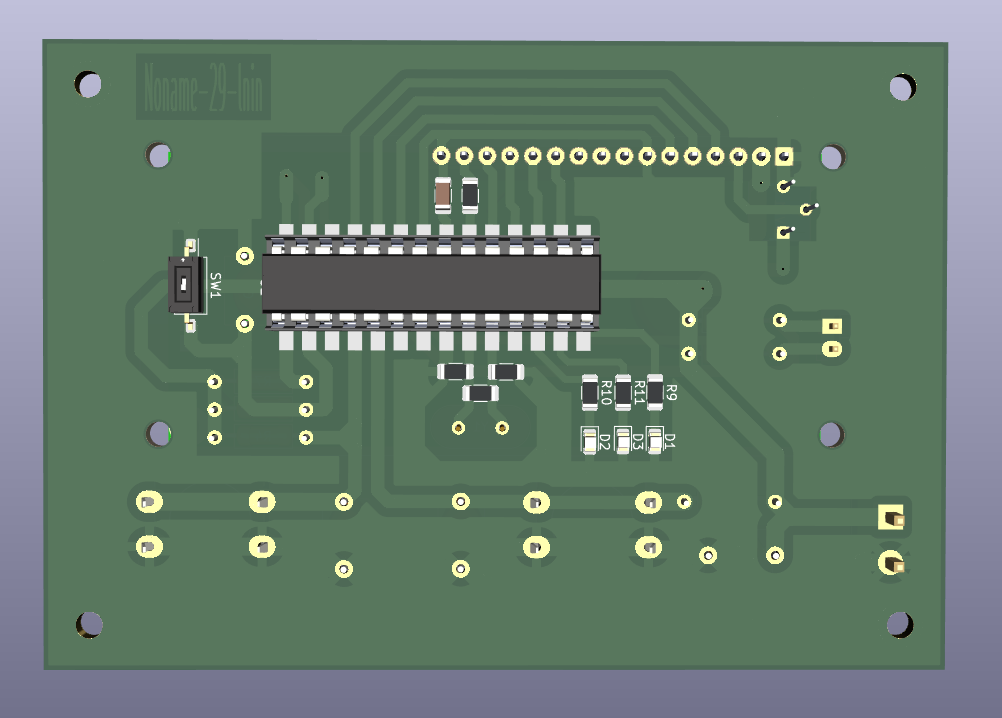
\includegraphics[width=\linewidth]{my-chapters/my-images/PCB_ADC/3D_underview.png}
	\end{minipage}
	\caption{3D của mạch đọc ADC.}
\end{figure}

\begin{figure}[H]
	\centering
	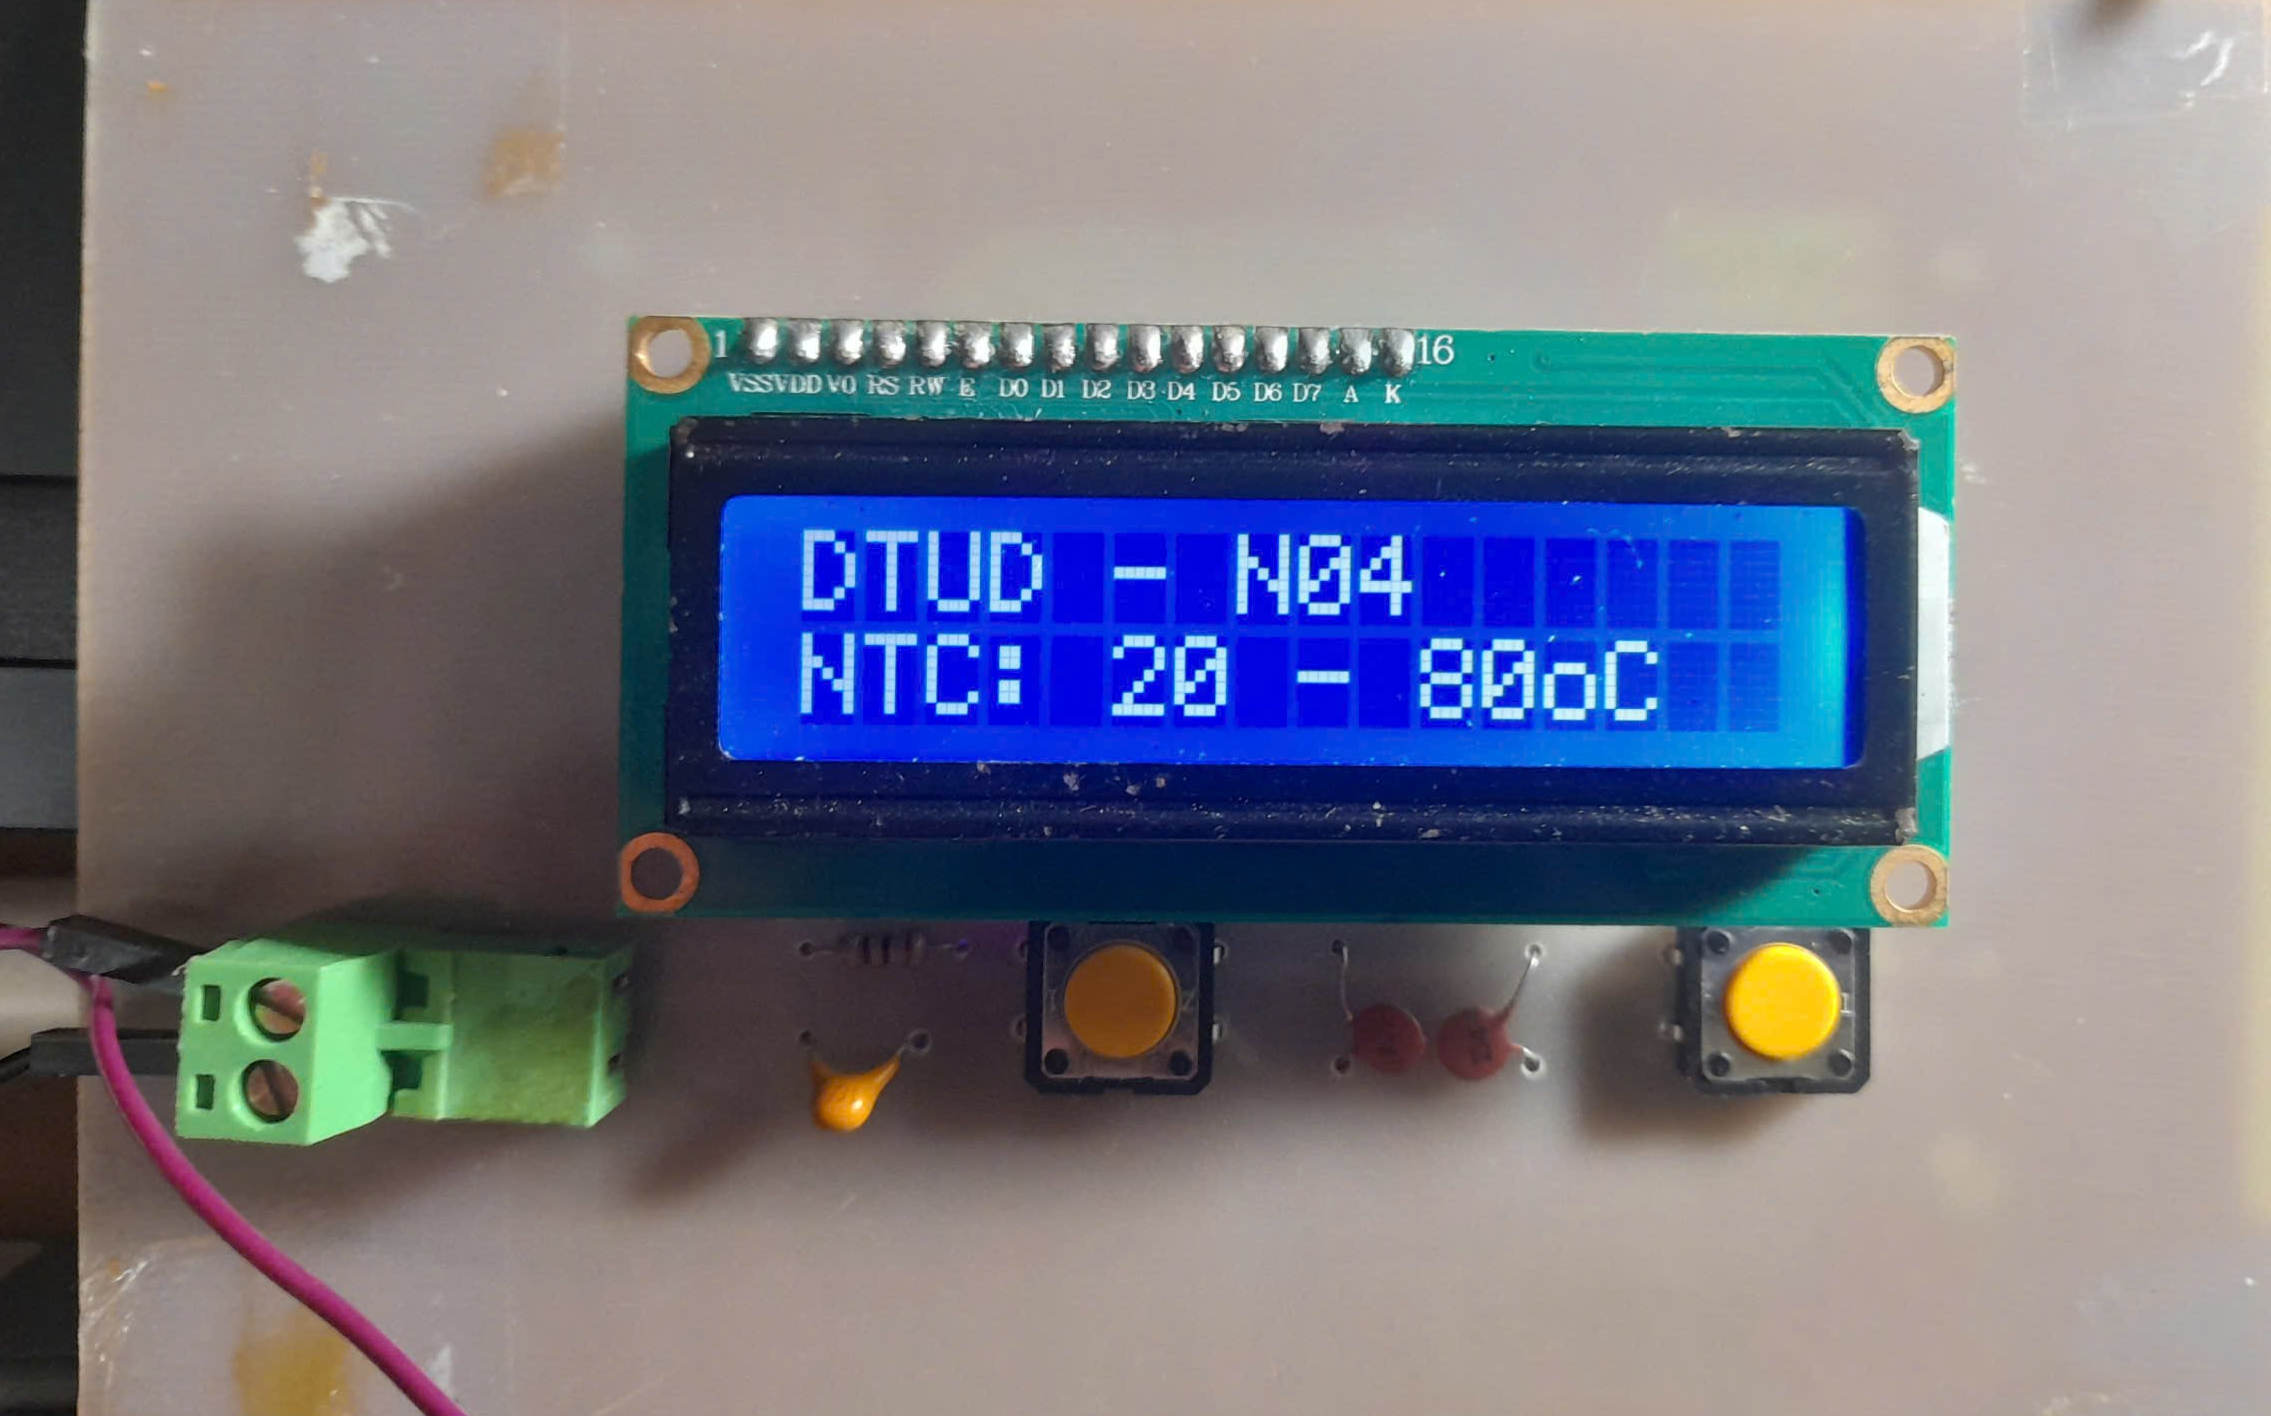
\includegraphics[width=.8\linewidth]{my-chapters/my-images/PCB_ADC/Real_ADCPCB.png}
	\caption{Mạch thực tế của mạch ADC.}
\end{figure}

\appendix
\section{Đoạn mã code của chương trình đọc nhiệt độ}
\lstinputlisting[style=StyleCode, language=C, caption={main\_ADC.c}]{./../ADC_code/main/main/main.c}
\lstinputlisting[style=StyleCode, language=C, caption={Func.h}]{./../ADC_code/main/main/Inc/Func.h}
\lstinputlisting[style=StyleCode, language=C, caption={Cal\_ADC.c}]{./../ADC_code/main/main/Src/Cal_ADC.c}
\lstinputlisting[style=StyleCode, language=C, caption={calib\_ADC.c}]{./../ADC_code/main/main/Src/calib.c}

\end{document}
